% =====================================================================
%  BÁO CÁO KỸ THUẬT — HỆ THỐNG BÃI ĐỖ XE THÔNG MINH
%  Môn: Lập trình nhúng (INT3108) — Trường ĐH Công nghệ, ĐHQGHN
%
%  Biên dịch (khuyến nghị XeLaTeX), tại thư mục report/:
%     xelatex bao_cao_smart_parking.tex   (chạy 2 lần để có mục lục)
%  hoặc:
%     tectonic bao_cao_smart_parking.tex
%  Trên Overleaf: tải cả thư mục report/ lên, Menu -> Compiler -> XeLaTeX.
%  Nội dung từng chương nằm trong report/chapters/.
% =====================================================================
\documentclass[12pt,a4paper]{report}

% ---------- Thông tin nhóm ----------
\newcommand{\tenmon}{Lập trình nhúng (INT3108)}
\newcommand{\tendetai}{Hệ thống bãi đỗ xe thông minh\\[2pt]sử dụng ESP32-C3 và ESP8266}
\newcommand{\giangvien}{Trần Hoàng Việt}
\newcommand{\lopmonhoc}{INT3108 1}
\newcommand{\thanhvien}{%
  Nguyễn Chí Minh & 24020232 \\
  Đinh Đức Thịnh & 24020313 \\
  Nguyễn Việt Tiến & 24020322 \\}
\newcommand{\repourl}{https://github.com/thinhdinh25/INT3108_embedded-Smart-Parking-Project}
% ------------------------------------

\usepackage{iftex}
\ifXeTeX
  \usepackage{fontspec}
  \setmainfont{texgyretermes}[Extension=.otf,UprightFont=*-regular,
    BoldFont=*-bold,ItalicFont=*-italic,BoldItalicFont=*-bolditalic]
  \setsansfont{texgyreheros}[Extension=.otf,UprightFont=*-regular,
    BoldFont=*-bold,ItalicFont=*-italic,BoldItalicFont=*-bolditalic]
  \setmonofont{texgyrecursor}[Extension=.otf,UprightFont=*-regular,
    BoldFont=*-bold,ItalicFont=*-italic,BoldItalicFont=*-bolditalic]
\else
  \usepackage[T5]{fontenc}
  \usepackage[utf8]{inputenc}
\fi
\usepackage[vietnamese,shorthands=off]{babel}

\usepackage[left=3cm,right=2cm,top=2.5cm,bottom=2.5cm]{geometry}
\usepackage{setspace}
\setstretch{1.25}
\usepackage{amsmath,amssymb}
\usepackage{graphicx}
\usepackage{xcolor}
\usepackage{booktabs,longtable,tabularx,array,multirow}
\usepackage{enumitem}
\setlist{itemsep=2pt,topsep=4pt}
\usepackage{float}
\usepackage{caption}
\captionsetup{font=small,labelfont=bf}
\usepackage{fancyhdr}
\usepackage{titlesec}
\usepackage{listings}
\usepackage{tikz}
\usetikzlibrary{arrows.meta,positioning,shapes.geometric,shapes.misc,fit,calc,backgrounds}
\usepackage{url}
\usepackage[hidelinks]{hyperref}

% Chữ và tiêu đề đen trắng; logo, mã nguồn, hình vẽ và hộp "Lý do" dùng màu.
\definecolor{uetblue}{gray}{0}
\definecolor{accent}{RGB}{0,62,126}
\definecolor{codebg}{RGB}{246,247,249}
\definecolor{codekw}{RGB}{0,82,163}
\definecolor{codecm}{RGB}{90,120,90}
\definecolor{codestr}{RGB}{163,21,21}
\definecolor{boxA}{RGB}{225,236,250}
\definecolor{boxB}{RGB}{232,245,233}
\definecolor{boxC}{RGB}{255,243,224}
\definecolor{boxD}{RGB}{252,228,236}
\definecolor{boxE}{RGB}{237,231,246}

\titleformat{\chapter}[hang]{\Large\bfseries\color{uetblue}}{Chương \thechapter.}{0.6em}{}
\titlespacing*{\chapter}{0pt}{-10pt}{14pt}
\titleformat{\section}{\large\bfseries\color{uetblue}}{\thesection}{0.6em}{}
\titleformat{\subsection}{\normalsize\bfseries}{\thesubsection}{0.6em}{}

\pagestyle{fancy}
\fancyhf{}
\fancyhead[L]{\small\itshape Báo cáo kỹ thuật — Bãi đỗ xe thông minh}
\fancyhead[R]{\small\itshape \tenmon}
\fancyfoot[C]{\thepage}
\renewcommand{\headrulewidth}{0.4pt}
\setlength{\headheight}{15pt}
\fancypagestyle{plain}{\fancyhf{}\fancyfoot[C]{\thepage}\renewcommand{\headrulewidth}{0pt}}

\lstset{
  basicstyle=\ttfamily\footnotesize,
  backgroundcolor=\color{codebg},
  keywordstyle=\color{codekw}\bfseries,
  commentstyle=\color{codecm}\itshape,
  stringstyle=\color{codestr},
  numbers=left, numberstyle=\tiny\color{gray}, numbersep=6pt,
  frame=single, rulecolor=\color{gray!40},
  breaklines=true, showstringspaces=false, tabsize=4,
  xleftmargin=1.5em, framexleftmargin=1.5em,
  captionpos=b, columns=fullflexible, keepspaces=true
}
\lstdefinelanguage{json}{
  morestring=[b]", stringstyle=\color{codestr},
  literate={:}{{\textcolor{codekw}{:}}}1 {,}{{\textcolor{codekw}{,}}}1
}
\lstdefinestyle{shell}{language=bash,numbers=none,backgroundcolor=\color{black!4},
  xleftmargin=0.5em,framexleftmargin=0.5em}
\renewcommand{\lstlistingname}{Mã nguồn}
\renewcommand{\lstlistlistingname}{Danh mục mã nguồn}

\newcommand{\codeus}{\textunderscore\allowbreak}
\newcommand{\code}[1]{{\ttfamily\let\_\codeus #1}}
\setlength{\emergencystretch}{3em}
\newcommand{\file}[1]{{\ttfamily\small\let\_\codeus #1}}

% Sơ đồ Mermaid (report/diagrams/*.mmd -> *.pdf, vector):
%   \mmd[tỉ lệ rộng][tỉ lệ cao tối đa]{tên}
% Tạo lại PDF: npx -p @mermaid-js/mermaid-cli mmdc -i diagrams/x.mmd -o diagrams/x.pdf -f
\NewDocumentCommand{\mmd}{O{1} O{0.6} m}{\includegraphics[width=#1\linewidth,height=#2\textheight,keepaspectratio]{diagrams/#3.pdf}}
% Hộp "Lý do lựa chọn" (có màu)
\usepackage[most]{tcolorbox}
\newtcolorbox{lydo}[1][Lý do lựa chọn]{breakable,enhanced,colback=boxA!55,
  colframe=accent,boxrule=0pt,leftrule=3pt,arc=0pt,outer arc=0pt,
  left=6pt,right=6pt,top=4pt,bottom=4pt,before skip=8pt,after skip=8pt,
  fonttitle=\bfseries,coltitle=accent,colbacktitle=boxA!55,
  title={#1},attach title to upper={.\ }}

% Đặc tả use case: nhãn bên trái, nội dung bên phải, ngắt trang tự nhiên
\newenvironment{usecase}[2]{%
  \par\medskip\noindent\rule{\linewidth}{0.8pt}\par\nobreak
  \noindent{\large\bfseries #1 — #2}\par\nobreak\vspace{-2pt}
  \noindent\rule{\linewidth}{0.4pt}\par\nobreak
  \begin{description}[style=multiline,leftmargin=3.3cm,font=\bfseries\normalsize,
    itemsep=3pt,topsep=2pt]}{%
  \end{description}\vspace{-4pt}\noindent\rule{\linewidth}{0.8pt}\par\medskip}

% Bước trong hướng dẫn chạy
\newcounter{buoc}
\newcommand{\buoc}[1]{\stepcounter{buoc}\par\medskip\noindent
  {\bfseries Bước \thebuoc.\ #1}\par\nobreak\smallskip}

\begin{document}

% =====================================================================
%  TRANG BÌA
% =====================================================================
\begin{titlepage}
  \centering
  \begin{tikzpicture}[remember picture,overlay]
    \draw[uetblue,line width=2pt] ($(current page.north west)+(2cm,-1.5cm)$)
      rectangle ($(current page.south east)+(-1.5cm,1.5cm)$);
    \draw[uetblue,line width=0.6pt] ($(current page.north west)+(2.15cm,-1.65cm)$)
      rectangle ($(current page.south east)+(-1.65cm,1.65cm)$);
  \end{tikzpicture}
  {\large ĐẠI HỌC QUỐC GIA HÀ NỘI\par}
  {\large\bfseries TRƯỜNG ĐẠI HỌC CÔNG NGHỆ\par}
  {\large\bfseries KHOA CÔNG NGHỆ THÔNG TIN\par}
  \vspace{0.4cm}
  \rule{0.5\linewidth}{0.8pt}\par
  \vspace{1.0cm}
  
\includegraphics[width=3.2cm]{uet_logo.png}\par
  \vspace{1.0cm}
  {\Large BÁO CÁO BÀI TẬP LỚN\par}
  \vspace{0.3cm}
  {\large Môn học: \tenmon\par}
  \vspace{1.4cm}
  {\LARGE\bfseries \tendetai\par}
  \vspace{1.6cm}
  \begin{tabular}{@{}ll@{}}
    \textbf{Giảng viên hướng dẫn:} & \giangvien \\
    \textbf{Lớp môn học:} & \lopmonhoc \\
  \end{tabular}
  \par\vspace{0.8cm}
  \textbf{Nhóm sinh viên thực hiện}\par\vspace{0.2cm}
  \begin{tabular}{|l|c|}
    \hline
    \textbf{Họ và tên} & \textbf{MSSV} \\ \hline
    \thanhvien
    \hline
  \end{tabular}
  \vfill
  {\large Hà Nội, tháng 10 năm 2026\par}
\end{titlepage}

% =====================================================================
\pagenumbering{roman}
\chapter*{Tóm tắt}
\addcontentsline{toc}{chapter}{Tóm tắt}

Báo cáo trình bày việc phân tích, thiết kế, hiện thực và kiểm thử một \textbf{hệ
thống bãi đỗ xe thông minh} quy mô mô hình gồm 5 chỗ đỗ và 2 cổng ra/vào. Hệ thống
gồm ba vi điều khiển Wi-Fi của Espressif phối hợp qua một mạng Wi-Fi cục bộ:

\begin{itemize}
  \item \textbf{Máy chủ} ESP32-C3 SuperMini chạy ESP-IDF 6.1 và hệ điều hành thời gian
        thực FreeRTOS: nhận dữ liệu qua UDP, quản lý phiên gửi xe và tính phí, điều
        khiển hai thanh chắn servo và còi báo cháy, hiển thị trên màn hình TFT ST7789
        và phục vụ trang web giám sát tại \code{http://parking.local} (mDNS).
  \item \textbf{Sensor Client} (ESP8266) đọc 5 cảm biến hồng ngoại, cảm biến lửa và
        cảm biến mực nước; gửi trạng thái ngay khi có thay đổi và nhắc lại mỗi giây.
  \item \textbf{RFID Client} (ESP8266) phát điểm truy cập Wi-Fi, đọc hai đầu đọc
        RFID MFRC522 (cổng vào, cổng ra) và cảm biến nhiệt độ DHT11.
\end{itemize}

Báo cáo đi theo đúng yêu cầu của môn học: giới thiệu bài toán, 10 use case chi
tiết, các thành phần hệ thống, hướng dẫn cài đặt môi trường, thiết kế và phân tích
kiến trúc (kèm demo), hướng dẫn chạy mã nguồn từng bước, kiểm thử, kết luận và phần
đóng góp của các thành viên. Mỗi lựa chọn công nghệ và thông số đều có hộp
\emph{Lý do} giải thích. Bộ kiểm thử tự động gồm 5 bộ với 250 phép kiểm tra chạy
trên máy tính — kể cả chạy lại chính mã nguồn Arduino của hai client trên phần cứng
giả lập — và đều đạt.

\medskip
\noindent\textbf{Từ khóa:} ESP32-C3, ESP8266, FreeRTOS, ESP-IDF, RFID, UDP, mDNS,
LEDC PWM, SPI DMA, ST7789, hệ thống nhúng thời gian thực.

\tableofcontents
\listoffigures
\listoftables
\lstlistoflistings

\chapter*{Danh mục từ viết tắt}
\addcontentsline{toc}{chapter}{Danh mục từ viết tắt}
\begin{longtable}{@{}p{2.6cm}p{11.5cm}@{}}
\toprule
\textbf{Viết tắt} & \textbf{Ý nghĩa} \\ \midrule
ADC & Analog-to-Digital Converter — bộ chuyển đổi tương tự–số \\
AP & Access Point — điểm truy cập Wi-Fi \\
API & Application Programming Interface \\
DHCP & Dynamic Host Configuration Protocol — cấp địa chỉ IP tự động \\
DMA & Direct Memory Access — truy cập bộ nhớ trực tiếp, không qua CPU \\
GPIO & General Purpose Input/Output \\
HTTP & HyperText Transfer Protocol \\
IDF & IoT Development Framework (ESP-IDF) \\
IR & Infrared — hồng ngoại \\
JSON & JavaScript Object Notation \\
LEDC & LED Control — khối phát PWM phần cứng của ESP32 \\
LZSS & Lempel–Ziv–Storer–Szymanski — thuật toán nén từ điển \\
mDNS & Multicast DNS — phân giải tên miền \code{.local} trong mạng cục bộ \\
NVS & Non-Volatile Storage — kho khóa–giá trị trên flash của ESP-IDF \\
OTA & Over-The-Air — nạp firmware qua mạng \\
PWM & Pulse Width Modulation — điều chế độ rộng xung \\
RFID & Radio Frequency Identification \\
RTOS & Real-Time Operating System \\
SPI & Serial Peripheral Interface \\
SSID & Service Set Identifier — tên mạng Wi-Fi \\
STA & Station — thiết bị kết nối vào một AP \\
TFT & Thin-Film Transistor (màn hình) \\
UC & Use case — ca sử dụng \\
UDP & User Datagram Protocol \\
UID & Unique Identifier — mã định danh của thẻ RFID \\
\bottomrule
\end{longtable}

\cleardoublepage
\pagenumbering{arabic}

% =====================================================================
\chapter{Giới thiệu bài toán}\label{chap:gioithieu}
% =====================================================================

\section{Bối cảnh}
Tại các đô thị lớn như Hà Nội, số lượng ô tô và xe máy tăng nhanh hơn nhiều so với
diện tích bãi đỗ. Người lái thường phải đi vòng nhiều lần để tìm chỗ trống, gây ùn
tắc cục bộ và lãng phí nhiên liệu. Phần lớn bãi xe hiện nay vẫn vận hành thủ công:
vé giấy, ghi biển số bằng tay, tính tiền bằng ước lượng, không biết trước còn bao
nhiêu chỗ và hầu như không có cơ chế cảnh báo an toàn khi xảy ra cháy hoặc ngập
nước — hai rủi ro thường gặp ở tầng hầm.

Một \textbf{bãi đỗ xe thông minh} tự động hóa các công việc này: cảm biến phát hiện
chỗ trống, thẻ RFID kiểm soát ra vào và tính phí, thanh chắn tự mở/đóng, cảm biến
môi trường cảnh báo sự cố và mọi thông tin được hiển thị trực tiếp tại bãi lẫn trên
điện thoại của người quản lý.

\section{Mục tiêu của bài toán}
Đề tài xây dựng một mô hình bãi xe 5 chỗ, 2 cổng, đáp ứng các mục tiêu:
\begin{enumerate}
  \item \textbf{Giám sát chỗ đỗ theo thời gian thực}: biết chính xác chỗ nào trống,
        chỗ nào có xe; màn hình tại bãi cập nhật trong khoảng 0,1 giây, trang web trong
        khoảng 1 giây.
  \item \textbf{Kiểm soát ra vào bằng thẻ RFID}: thẻ quẹt ở cổng vào mở thanh chắn
        vào, cùng thẻ quẹt ở cổng ra mở thanh chắn ra; thanh chắn tự đóng sau 3 giây;
        quẹt sai cổng hoặc bãi đầy bị từ chối và thông báo rõ trên màn hình.
  \item \textbf{Tính phí tự động}: 5.000\,VNĐ cho mỗi giờ bắt đầu, tối thiểu 1 giờ;
        hiển thị hóa đơn khi xe ra.
  \item \textbf{An toàn}: phát hiện lửa — bật còi, hiển thị cảnh báo, \emph{mở cả hai
        thanh chắn} để sơ tán; theo dõi mực nước và nhiệt độ.
  \item \textbf{Giám sát và điều khiển từ xa}: trang web tại \code{http://parking.local}
        dùng được trên mọi điện thoại, không cần cài ứng dụng, có nhật ký xe vào/ra.
  \item \textbf{Hoạt động độc lập}: tự tạo mạng Wi-Fi riêng, không cần Internet hay
        router; tự phục hồi khi mất kết nối.
\end{enumerate}

\section{Ý nghĩa}
\paragraph{Ý nghĩa thực tiễn.} Mô hình chứng minh rằng một bãi xe nhỏ (chung cư mini,
văn phòng, trường học) có thể được tự động hóa bằng linh kiện phổ thông giá rẻ.
Người lái biết ngay còn chỗ hay không; người quản lý thu phí chính xác, có nhật ký
xe ra vào, được cảnh báo cháy/ngập kịp thời; khi cháy, thanh chắn tự mở giúp sơ tán
nhanh.

\paragraph{Ý nghĩa học thuật.} Đây là bài toán nhúng điển hình, vận dụng gần như toàn
bộ kiến thức của môn học: lập trình đa tác vụ với \textbf{hệ điều hành thời gian
thực FreeRTOS}, đồng bộ giữa các tác vụ, điều khiển ngoại vi bằng phần cứng chuyên
dụng (PWM, SPI có DMA, ADC, GPIO), giao tiếp không dây, quản lý bộ nhớ hạn chế
(vài trăm KB RAM), xử lý dữ liệu không tin cậy từ mạng và kiểm thử phần mềm nhúng
khi không có phần cứng.

\section{Phạm vi}
Hệ thống là \textbf{mô hình} quy mô phòng thí nghiệm: 5 chỗ đỗ, 2 cổng, xe mô hình,
thẻ RFID MIFARE. Thanh toán điện tử, nhận dạng biển số và lưu trữ đám mây nằm ngoài
phạm vi và được nêu ở phần hướng phát triển (Chương~\ref{chap:ketluan}).

\section{Kết quả đạt được (tóm tắt)}
\begin{itemize}
  \item Ba bo mạch hoạt động phối hợp, 10 use case (Chương~\ref{chap:usecase}) đều
        được hiện thực và có phép kiểm thử tương ứng.
  \item Firmware máy chủ 1,08\,MB, dùng 36\% RAM tĩnh; còn 29\% phân vùng ứng dụng.
  \item 250 phép kiểm thử tự động đều đạt (Chương~\ref{chap:kiemthu}).
\end{itemize}

\section{Cấu trúc báo cáo}
\begin{table}[H]
\centering\small
\caption{Cấu trúc báo cáo theo yêu cầu của môn học}\label{tab:cautruc}
\begin{tabularx}{\linewidth}{@{}lXl@{}}
\toprule
\textbf{Chương} & \textbf{Nội dung} & \textbf{Yêu cầu} \\ \midrule
\ref{chap:gioithieu} & Giới thiệu bài toán, mục tiêu, ý nghĩa & Giới thiệu (1đ) \\
\ref{chap:usecase} & 10 use case: tác nhân, luồng chính, ngoại lệ, kiểm thử & Use case (10đ) \\
\ref{chap:thanhphan} & Các thành phần phần cứng và phần mềm, thông số quan trọng & Thành phần (2đ) \\
\ref{chap:caidat} & Cài đặt môi trường, hệ điều hành, phần mềm mô phỏng & Cài đặt (1đ) \\
\ref{chap:thietke} & Thiết kế, phân tích kiến trúc, luồng hoạt động, demo & Thiết kế (3đ) \\
\ref{chap:huongdanchay} & Hướng dẫn chạy mã nguồn từng bước & Chạy mã nguồn (2đ) \\
\ref{chap:kiemthu} & Kiểm thử tự động và kịch bản kiểm thử phần cứng & Bổ trợ thiết kế/demo \\
\ref{chap:ketluan} & Tổng kết, hạn chế, hướng phát triển & Kết luận (1đ) \\
\ref{chap:donggop} & Đóng góp của thành viên, phân chia điểm & Đóng góp \\
\bottomrule
\end{tabularx}
\end{table}

% =====================================================================
\chapter{Use case của hệ thống}\label{chap:usecase}
% =====================================================================

\section{Tác nhân}
\begin{table}[H]
\centering\small
\caption{Các tác nhân của hệ thống}\label{tab:actors}
\begin{tabularx}{\linewidth}{@{}lX@{}}
\toprule
\textbf{Tác nhân} & \textbf{Mô tả} \\ \midrule
Người lái xe & Người gửi/lấy xe; dùng thẻ RFID và nhìn màn hình TFT tại bãi. \\
Người vận hành & Bảo vệ hoặc quản lý bãi; dùng trang web trên điện thoại/máy tính để giám sát và điều khiển thanh chắn. \\
Sensor Client & Tác nhân thiết bị: bo ESP8266 đọc cảm biến chỗ đỗ, lửa, nước và gửi dữ liệu lên máy chủ. \\
RFID Client & Tác nhân thiết bị: bo ESP8266 đọc thẻ ở hai cổng và cảm biến nhiệt độ; đồng thời phát mạng Wi-Fi. \\
Đồng hồ hệ thống & Tác nhân thời gian: kích hoạt việc tự đóng thanh chắn, hết hạn hóa đơn/thông báo. \\
\bottomrule
\end{tabularx}
\end{table}

\section{Sơ đồ use case}
Hình~\ref{fig:usecase} tổng hợp 10 use case và quan hệ với các tác nhân. Hai tác nhân
thiết bị (bên phải) là nguồn dữ liệu; hai tác nhân con người (bên trái) là người
hưởng lợi.

\begin{figure}[H]
\centering
\mmd[1][0.62]{usecase}
\caption{Sơ đồ use case tổng quát (đường nét đứt: sự kiện theo thời gian — tự đóng thanh chắn, hết hạn thông báo)}\label{fig:usecase}
\end{figure}

\section{Bảng tổng hợp use case}
\begin{table}[H]
\centering\small
\caption{Tổng hợp 10 use case, nơi hiện thực và bộ kiểm thử tương ứng}\label{tab:uc-summary}
\begin{tabularx}{\linewidth}{@{}l>{\raggedright\arraybackslash}p{4.2cm}>{\raggedright\arraybackslash}X>{\raggedright\arraybackslash}p{3.1cm}@{}}
\toprule
\textbf{Mã} & \textbf{Tên use case} & \textbf{Module chính} & \textbf{Kiểm thử} \\ \midrule
UC01 & Theo dõi chỗ trống tại bãi & \file{lcd\_display.c} & \file{sensor\_client} \\
UC02 & Giám sát bãi qua web & \file{http\_server.c}, \file{index.html} & S2, S12 \\
UC03 & Gửi xe bằng thẻ RFID & \file{rfid\_session.c}, \file{servo.c} & \file{rfid\_session}, \file{rfid\_client} \\
UC04 & Lấy xe và thanh toán phí & \file{rfid\_session.c} & \file{rfid\_session} \\
UC05 & Từ chối quẹt sai cổng / bãi đầy & \file{rfid\_session.c}, \file{lcd\_display.c} & \file{rfid\_session} \\
UC06 & Cảnh báo cháy và sơ tán & \file{udp\_server.c}, \file{servo.c}, \file{buzzer.c} & \file{sensor\_client}, S9 \\
UC07 & Giám sát mực nước & \file{SensorClient.ino} & \file{sensor\_client} \\
UC08 & Giám sát nhiệt độ & \file{RFIDClient.ino}, \file{parking\_state.c} & \file{rfid\_client}, \file{rfid\_session} \\
UC09 & Điều khiển thanh chắn thủ công & \file{http\_server.c}, \file{servo.c} & S12, S13 \\
UC10 & Xem nhật ký vào/ra và giá & \file{rfid\_session.c}, \file{http\_server.c} & \file{rfid\_session} \\
\bottomrule
\end{tabularx}
\end{table}
\noindent Tên tệp kiểm thử như \file{rfid\_session} chỉ bộ kiểm thử tự động
(Chương~\ref{chap:kiemthu}); S2, S9,\ldots{} là kịch bản kiểm thử trên phần cứng
(Bảng~\ref{tab:systest}).

\section{Đặc tả chi tiết}

\begin{usecase}{UC01}{Theo dõi chỗ trống tại bãi}
\item[Tác nhân] Người lái xe (chính); Sensor Client (nguồn dữ liệu).
\item[Mô tả] Người lái nhìn màn hình TFT ở lối vào để biết số chỗ trống và vị trí từng chỗ trống.
\item[Tiền điều kiện] Sensor Client và máy chủ đã kết nối Wi-Fi \code{ESP32-Parking}.
\item[Luồng chính] \begin{enumerate}[nosep,leftmargin=1.3em]
  \item Xe đi vào/ra một ô đỗ, cảm biến IR của ô đó đổi mức logic.
  \item Sensor Client lọc nhiễu: chỉ chấp nhận mức mới khi giữ ổn định 50\,ms.
  \item Ngay khi trạng thái đổi, Sensor Client gửi bản tin \code{parking\_update} (UDP).
  \item Máy chủ kiểm tra bản tin, cập nhật trạng thái chung và đánh thức tác vụ màn hình.
  \item Màn hình vẽ lại: số chỗ trống \code{FREE SPACES x/5} và 5 ô S1–S5 (xanh = trống, đỏ = có xe).
\end{enumerate}
\item[Ngoại lệ] 3a. Mất gói UDP: bản tin nhắc lại sau tối đa 1\,s sửa lại trạng thái.
  4a. Bản tin sai định dạng: bị bỏ qua, trạng thái cũ được giữ.
\item[Hậu điều kiện] Màn hình phản ánh đúng trạng thái 5 chỗ đỗ.
\item[Thông số] Debounce 50\,ms; nhắc lại 1\,s; độ trễ hiển thị $\approx$ 0,1\,s.
\end{usecase}

\begin{usecase}{UC02}{Giám sát bãi qua trang web}
\item[Tác nhân] Người vận hành.
\item[Mô tả] Xem trực quan sơ đồ bãi, số chỗ trống, cảm biến và trạng thái thanh chắn trên điện thoại.
\item[Tiền điều kiện] Thiết bị của người vận hành kết nối Wi-Fi \code{ESP32-Parking}.
\item[Luồng chính] \begin{enumerate}[nosep,leftmargin=1.3em]
  \item Người vận hành mở \code{http://parking.local}.
  \item Thiết bị phân giải tên bằng mDNS và nhận địa chỉ IP hiện tại của máy chủ.
  \item Máy chủ trả trang web nhúng trong firmware.
  \item Trang web gọi \code{GET /api/parking} mỗi 1\,s và vẽ sơ đồ 5 ô đỗ (xe màu đỏ, ô trống chữ P màu xanh).
\end{enumerate}
\item[Ngoại lệ] 2a. Thiết bị không hỗ trợ \code{.local}: dùng địa chỉ IP in trên log máy chủ.
  4a. Máy chủ mất kết nối: trang hiển thị \code{ESP32 / OFFLINE}.
\item[Hậu điều kiện] Người vận hành thấy trạng thái bãi với độ trễ $\le$ 1\,s.
\end{usecase}

\begin{usecase}{UC03}{Gửi xe bằng thẻ RFID}
\item[Tác nhân] Người lái xe; RFID Client; Đồng hồ hệ thống.
\item[Mô tả] Người lái quẹt thẻ ở cổng vào để được mở thanh chắn và bắt đầu tính giờ.
\item[Tiền điều kiện] Thẻ chưa có phiên gửi xe; bãi còn phiên trống (tối đa 5).
\item[Luồng chính] \begin{enumerate}[nosep,leftmargin=1.3em]
  \item Người lái đưa thẻ vào đầu đọc cổng vào.
  \item RFID Client đọc UID, chuyển thành chuỗi hex in hoa, gửi \code{rfid\_event} với \code{"gate":"in"}.
  \item Máy chủ tạo phiên mới, lưu thời điểm vào, ghi nhật ký \code{IN}.
  \item Máy chủ mở thanh chắn cổng vào (90°) và hẹn giờ đóng sau 3\,s.
  \item Đồng hồ hết 3\,s, thanh chắn tự đóng.
\end{enumerate}
\item[Ngoại lệ] 1a. Thẻ để yên trên đầu đọc: chỉ gửi một lần trong 2\,s.
  3a. Bãi đầy hoặc thẻ đã ở trong bãi: chuyển sang UC05.
  5a. Người vận hành bấm đóng/mở trên web trước khi hết giờ: lệnh tay thắng, hủy hẹn giờ.
\item[Hậu điều kiện] Thẻ có phiên hoạt động; thanh chắn đóng lại.
\item[Thông số] Thời gian mở 3\,s; chống đọc lặp 2\,s; tối đa 5 phiên.
\end{usecase}

\begin{usecase}{UC04}{Lấy xe và thanh toán phí}
\item[Tác nhân] Người lái xe; RFID Client; Đồng hồ hệ thống.
\item[Mô tả] Người lái quẹt cùng thẻ ở cổng ra; hệ thống tính phí, hiển thị hóa đơn và mở cổng ra.
\item[Tiền điều kiện] Thẻ đang có phiên gửi xe.
\item[Luồng chính] \begin{enumerate}[nosep,leftmargin=1.3em]
  \item Người lái quẹt thẻ ở đầu đọc cổng ra (\code{"gate":"out"}).
  \item Máy chủ tính thời gian gửi $t$ và phí $\max(1,\lceil t/3600\rceil)\times5000$\,VNĐ.
  \item Máy chủ đóng phiên, ghi nhật ký \code{OUT} kèm thời gian và phí.
  \item Màn hình hiển thị hóa đơn: UID, \code{PARK TIME}, \code{FEE VND} trong 60\,s.
  \item Thanh chắn cổng ra mở và tự đóng sau 3\,s.
\end{enumerate}
\item[Ngoại lệ] 1a. Thẻ chưa vào bãi: chuyển sang UC05.
\item[Hậu điều kiện] Phiên được giải phóng; nhật ký có bản ghi \code{OUT}.
\item[Thông số] 5.000\,VNĐ/giờ, làm tròn lên, tối thiểu 1 giờ; hóa đơn hiển thị 60\,s.
\end{usecase}

\begin{usecase}{UC05}{Từ chối quẹt sai cổng / bãi đầy}
\item[Tác nhân] Người lái xe; RFID Client; Đồng hồ hệ thống.
\item[Mô tả] Hệ thống từ chối các lần quẹt không hợp lệ và hướng dẫn người lái.
\item[Tiền điều kiện] Một trong ba trường hợp: (a) thẻ đã trong bãi nhưng quẹt ở cổng vào;
  (b) thẻ chưa vào nhưng quẹt ở cổng ra; (c) đã đủ 5 phiên mà có thẻ mới ở cổng vào.
\item[Luồng chính] \begin{enumerate}[nosep,leftmargin=1.3em]
  \item Máy chủ nhận \code{rfid\_event} và xác định kết quả \code{INVALID\_GATE} hoặc \code{FULL}.
  \item Thanh chắn \emph{không} mở.
  \item Màn hình hiển thị thông báo đỏ trong 5\,s: \code{WRONG GATE} kèm gợi ý
        \code{ALREADY INSIDE - USE EXIT GATE} / \code{NOT CHECKED IN - USE ENTRY GATE},
        hoặc \code{PARKING FULL}.
  \item Nhật ký ghi \code{REJECTED · WRONG GATE} hoặc \code{REJECTED · FULL}.
\end{enumerate}
\item[Ngoại lệ] 3a. Đang hiển thị hóa đơn: thông báo hiện trước, hết 5\,s hóa đơn hiện lại.
  3b. Ngay sau đó có lần quẹt hợp lệ: thông báo cũ bị xóa ngay.
\item[Hậu điều kiện] Trạng thái phiên không đổi.
\end{usecase}

\begin{usecase}{UC06}{Cảnh báo cháy và sơ tán}
\item[Tác nhân] Sensor Client (cảm biến lửa); Người lái xe; Người vận hành.
\item[Mô tả] Khi phát hiện lửa: báo động tại chỗ, trên web và mở thanh chắn để sơ tán.
\item[Tiền điều kiện] Sensor Client đang gửi dữ liệu.
\item[Luồng chính] \begin{enumerate}[nosep,leftmargin=1.3em]
  \item Cảm biến lửa phát hiện ngọn lửa ổn định quá 50\,ms; Sensor Client gửi ngay \code{"fire":true}.
  \item Máy chủ bật còi (GPIO9 mức thấp).
  \item Máy chủ chuyển \emph{chế độ cháy}: mở cả hai thanh chắn và giữ mở.
  \item Màn hình chuyển sang màn hình \code{DANGER / FIRE DETECTED / EVACUATE NOW} có ngọn lửa động.
  \item Trang web hiện băng rôn đỏ \code{FIRE DETECTED}.
\end{enumerate}
\item[Ngoại lệ] 3a. Người vận hành bấm đóng thanh chắn: bị từ chối (HTTP 500) trong chế độ cháy.
  6a. Hết lửa (\code{"fire":false}): tắt còi, đóng cả hai thanh chắn, màn hình trở lại bình thường.
\item[Hậu điều kiện] Lối ra vào thông thoáng trong suốt thời gian có lửa.
\end{usecase}

\begin{usecase}{UC07}{Giám sát mực nước}
\item[Tác nhân] Sensor Client; Người vận hành.
\item[Mô tả] Theo dõi mực nước ngập tại bãi (mô hình tầng hầm).
\item[Luồng chính] \begin{enumerate}[nosep,leftmargin=1.3em]
  \item Sensor Client đọc ADC chân A0 mỗi 250\,ms.
  \item Quy đổi tuyến tính ADC 20–700 thành 0–40\,mm (giới hạn trên 40\,mm).
  \item Giá trị được gửi trong \code{parking\_update}; máy chủ kiểm tra dải 0–10.000\,mm.
  \item Màn hình (\code{WATER MM}) và web (\code{WATER LEVEL}) hiển thị giá trị.
\end{enumerate}
\item[Ngoại lệ] 3a. Giá trị âm hoặc vượt dải: bản tin bị từ chối.
\item[Hậu điều kiện] Mực nước hiển thị với độ phân giải 0,1\,mm.
\end{usecase}

\begin{usecase}{UC08}{Giám sát nhiệt độ}
\item[Tác nhân] RFID Client (DHT11); Người vận hành.
\item[Mô tả] Theo dõi nhiệt độ môi trường tại cổng.
\item[Luồng chính] \begin{enumerate}[nosep,leftmargin=1.3em]
  \item RFID Client đọc DHT11 mỗi 5\,s, giữ giá trị hợp lệ gần nhất.
  \item Giá trị được gửi kèm mỗi \code{rfid\_event} (\code{temperature\_c}).
  \item Máy chủ kiểm tra dải $-40$ đến $125$\,°C, cập nhật trạng thái chung.
  \item Màn hình (\code{TEMP C}) và web (\code{TEMPERATURE}) hiển thị.
\end{enumerate}
\item[Ngoại lệ] 1a. DHT11 đọc lỗi (NaN): giữ giá trị cũ, không gửi số sai.
\item[Hậu điều kiện] Nhiệt độ cập nhật mỗi lần có xe quẹt thẻ.
\end{usecase}

\begin{usecase}{UC09}{Điều khiển thanh chắn thủ công}
\item[Tác nhân] Người vận hành.
\item[Mô tả] Mở/đóng từng thanh chắn hoặc cả hai (khẩn cấp) từ trang web.
\item[Luồng chính] \begin{enumerate}[nosep,leftmargin=1.3em]
  \item Người vận hành bấm \code{OPEN}/\code{CLOSE} của cổng vào, cổng ra, hoặc
        \code{EMERGENCY OPEN/CLOSE ALL}.
  \item Trang web gửi yêu cầu \code{POST} tới \code{/api/barrier/<cổng>/<lệnh>} (cổng: \code{in}, \code{out}, \code{all}; lệnh: \code{open}, \code{close}); nút bị khóa đến khi có phản hồi.
  \item Máy chủ hủy hẹn giờ tự đóng (nếu có) rồi đặt góc servo.
  \item Trang web cập nhật trạng thái \code{OPEN}/\code{CLOSED}.
\end{enumerate}
\item[Ngoại lệ] 3a. Đang có cháy mà yêu cầu đóng: từ chối, hiển thị lỗi.
\item[Hậu điều kiện] Thanh chắn ở đúng trạng thái người vận hành chọn.
\end{usecase}

\begin{usecase}{UC10}{Xem nhật ký vào/ra và giá gửi xe}
\item[Tác nhân] Người vận hành.
\item[Mô tả] Biết ai đang trong bãi, đã gửi bao lâu, phí tạm tính, và 10 sự kiện gần nhất.
\item[Luồng chính] \begin{enumerate}[nosep,leftmargin=1.3em]
  \item Trang web gọi \code{GET /api/rfid} mỗi 2\,s.
  \item Máy chủ trả giá mỗi giờ, danh sách xe trong bãi (UID, giờ vào, phí tạm tính) và
        10 sự kiện mới nhất (vào, ra kèm thời lượng và phí, bị từ chối).
  \item Trình duyệt đổi thời gian ``giây kể từ khi khởi động'' thành giờ thực theo đồng hồ điện thoại.
\end{enumerate}
\item[Ngoại lệ] 2a. Máy chủ khởi động lại: nhật ký và phiên được làm mới (lưu trong RAM).
\item[Hậu điều kiện] Người vận hành đối soát được tiền thu và xe trong bãi.
\end{usecase}

% =====================================================================
\chapter{Các thành phần hệ thống}\label{chap:thanhphan}
% =====================================================================

Chương này liệt kê mọi thành phần phần cứng và phần mềm của hệ thống, kèm các thông
số quan trọng quyết định thiết kế. Lý do chọn từng thành phần được trình bày trong
các hộp \emph{Lý do}; phần kiến trúc tổng thể nằm ở Chương~\ref{chap:thietke}.

\section{Tổng quan ba nút phần cứng}
\begin{table}[H]
\centering\small
\caption{Ba nút phần cứng và vai trò}\label{tab:nodes}
\begin{tabularx}{\linewidth}{@{}lXl@{}}
\toprule
\textbf{Nút} & \textbf{Thiết bị gắn kèm và nhiệm vụ} & \textbf{Mã nguồn} \\ \midrule
Máy chủ (ESP32-C3) & TFT ST7789, 2 servo SG90, còi. Nhận UDP, quản lý phiên RFID, tính phí, điều khiển thanh chắn, web server, mDNS & \file{Server/main/} \\
Sensor Client (ESP8266) & 5 cảm biến IR, cảm biến lửa, cảm biến mực nước. Lọc nhiễu và gửi trạng thái & \file{SensorClient/} \\
RFID Client (ESP8266) & 2 đầu đọc MFRC522, DHT11. Phát Wi-Fi, gửi sự kiện quẹt thẻ & \file{RFIDClient/} \\
\bottomrule
\end{tabularx}
\end{table}

\section{Vi điều khiển}
\subsection{ESP32-C3 SuperMini (máy chủ)}
\begin{table}[H]
\centering\small
\caption{Thông số quan trọng của ESP32-C3 SuperMini}\label{tab:esp32c3}
\begin{tabularx}{\linewidth}{@{}lX@{}}
\toprule
CPU & RISC-V 32 bit, 1 nhân, chạy ở 160\,MHz \\
Bộ nhớ & 400\,KB SRAM (ứng dụng dùng được $\approx$ 321\,KB DRAM), 384\,KB ROM \\
Flash & Flash ngoài, cấu hình 2\,MB; phân vùng ứng dụng 1,5\,MB \\
Không dây & Wi-Fi 802.11 b/g/n 2,4\,GHz, Bluetooth LE 5 \\
Ngoại vi dùng tới & SPI2 có GDMA, LEDC (PWM 14 bit), GPIO, bộ định thời \code{esp\_timer} 64 bit \\
Nạp/gỡ lỗi & USB Serial/JTAG tích hợp (không cần chip USB-UART, không cần driver) \\
Kích thước & $22\times18$\,mm \\
\bottomrule
\end{tabularx}
\end{table}

\begin{table}[H]
\centering\small
\caption{So sánh phương án vi điều khiển cho máy chủ}\label{tab:mcu}
\begin{tabularx}{\linewidth}{@{}lXXXX@{}}
\toprule
\textbf{Tiêu chí} & \textbf{ESP32-C3} & \textbf{ESP32} & \textbf{ESP8266} & \textbf{Arduino Uno} \\ \midrule
CPU & RISC-V 160\,MHz & Xtensa 2 nhân 240\,MHz & Xtensa 80/160\,MHz & AVR 16\,MHz \\
SRAM & 400\,KB & 520\,KB & $\sim$80\,KB & 2\,KB \\
Wi-Fi & Có & Có & Có & Không \\
PWM phần cứng & LEDC 14 bit & LEDC & PWM mềm & 8 bit \\
SPI có DMA & Có & Có & Hạn chế & Không \\
RTOS chính thức & FreeRTOS & FreeRTOS & Hạn chế & Không \\
\bottomrule
\end{tabularx}
\end{table}

\begin{lydo}
Máy chủ phải \emph{đồng thời} giữ Wi-Fi, chạy web server và UDP server, vẽ màn hình
$240\times240$ màu 16 bit và phát PWM cho servo. Chỉ riêng ảnh màn hình đã cần
$240\times240\times2 = 115\,200$ byte RAM — lớn hơn toàn bộ RAM của ESP8266 hay
Arduino. ESP32-C3 có đủ RAM, có DMA cho SPI (CPU không phải chờ khi đẩy ảnh), có PWM
phần cứng (servo không rung khi CPU bận mạng) và được hỗ trợ chính thức bởi
ESP-IDF/FreeRTOS. So với ESP32 bản gốc, C3 rẻ và nhỏ hơn; một nhân 160\,MHz đã dư
năng lực cho bài toán này.
\end{lydo}

\subsection{ESP8266 NodeMCU (hai client)}
\begin{table}[H]
\centering\small
\caption{Thông số quan trọng của ESP8266}\label{tab:esp8266}
\begin{tabularx}{\linewidth}{@{}lX@{}}
\toprule
CPU & Tensilica L106 32 bit, 80\,MHz \\
Bộ nhớ & $\sim$80\,KB RAM dữ liệu cho người dùng, flash 4\,MB trên bo NodeMCU \\
Ngoại vi dùng tới & 1 kênh ADC 10 bit (A0), SPI phần cứng (HSPI), GPIO \\
Không dây & Wi-Fi 802.11 b/g/n, chạy được chế độ STA hoặc AP \\
\bottomrule
\end{tabularx}
\end{table}

\begin{lydo}
Nút cảm biến chỉ đọc vài chân số, một chân ADC, giao tiếp SPI với RC522 và gửi gói
UDP nhỏ — nhu cầu tính toán rất thấp. ESP8266 là bo Wi-Fi rẻ và phổ biến nhất, có
ADC, có hệ sinh thái thư viện Arduino lớn (MFRC522, DHT, ArduinoOTA). Tách ra hai
bo vì máy chủ không đủ chân: màn hình, servo và còi đã dùng 9 chân trong khoảng 13
chân khả dụng của ESP32-C3 SuperMini.
\end{lydo}

\section{Thiết bị chấp hành và hiển thị}
\begin{table}[H]
\centering\small
\caption{Thiết bị chấp hành, hiển thị và thông số quan trọng}\label{tab:actuators}
\begin{tabularx}{\linewidth}{@{}p{3.1cm}X@{}}
\toprule
\textbf{Thiết bị} & \textbf{Thông số quan trọng} \\ \midrule
TFT ST7789 1,54" & $240\times240$, IPS, 262K màu (dùng RGB565 16 bit), SPI chỉ ghi, chu kỳ ghi tối thiểu $\approx$ 16\,ns ($\approx$ 62\,MHz); hệ thống chạy 40\,MHz \\
Servo SG90 $\times2$ & 4,8–6\,V; mô-men $\approx$ 1,8\,kg$\cdot$cm; tốc độ $\approx$ 0,1\,s/60°; điều khiển PWM 50\,Hz, xung $\approx$ 500–2400\,µs cho 0–180° \\
Còi (module) & Tích cực mức thấp: chân tín hiệu mức 0 thì kêu \\
\bottomrule
\end{tabularx}
\end{table}

\section{Cảm biến}
\begin{table}[H]
\centering\small
\caption{Cảm biến, thông số và lý do lựa chọn}\label{tab:sensors}
\begin{tabularx}{\linewidth}{@{}p{2.9cm}p{4.0cm}X@{}}
\toprule
\textbf{Cảm biến} & \textbf{Thông số} & \textbf{Lý do lựa chọn} \\ \midrule
IR phản xạ HW-201 (họ FC-51) $\times5$ & 2–30\,cm, so sánh LM393 có biến trở, ngõ ra số tích cực mức thấp & Rẻ, phát hiện vật ở cự ly vài cm hợp với xe mô hình, chỉ tốn 1 chân. Siêu âm chính xác hơn nhưng tốn 2 chân/cảm biến và phải đo thời gian. \\
Cảm biến lửa (module 4 chân AO/DO) & Bước sóng 760–1100\,nm, góc $\approx$ 60°, ngõ ra số có ngưỡng & Phản ứng nhanh hơn cảm biến khói/nhiệt; ngõ ra số sẵn ngưỡng. \\
Mực nước (điện trở) & Vùng đo $\approx$ 40\,mm, ngõ ra tương tự & Đơn giản, chỉ cần 1 chân ADC, hợp với mô hình tầng hầm. \\
RFID MFRC522 $\times2$ & 13,56\,MHz, ISO 14443A (MIFARE), SPI, 3,3\,V, đọc vài cm & Đọc được thẻ phổ biến (thẻ sinh viên, móc khóa), thư viện ổn định, giá rẻ. \\
DHT11 & 0–50\,°C ($\pm$2\,°C), 20–90\%RH, đọc tối đa 1 lần/giây & Đủ cho giám sát môi trường, chỉ cần 1 chân. \\
\bottomrule
\end{tabularx}
\end{table}

\section{Mô hình thực tế và bố trí phần cứng}\label{sec:mohinh}
Hình~\ref{fig:model} là mô hình nhóm đã chế tạo. Đế và vách làm bằng bìa formex
trắng (nhẹ, dễ cắt khoét lỗ cho cảm biến, cách điện); 5 ô đỗ được kẻ vạch dọc vách
sau, phía trước là sân quay đầu và hai làn ra/vào nằm hai bên hộp điều khiển ở giữa.

\begin{figure}[H]
\centering
\begin{subfigure}[t]{0.49\linewidth}\centering
  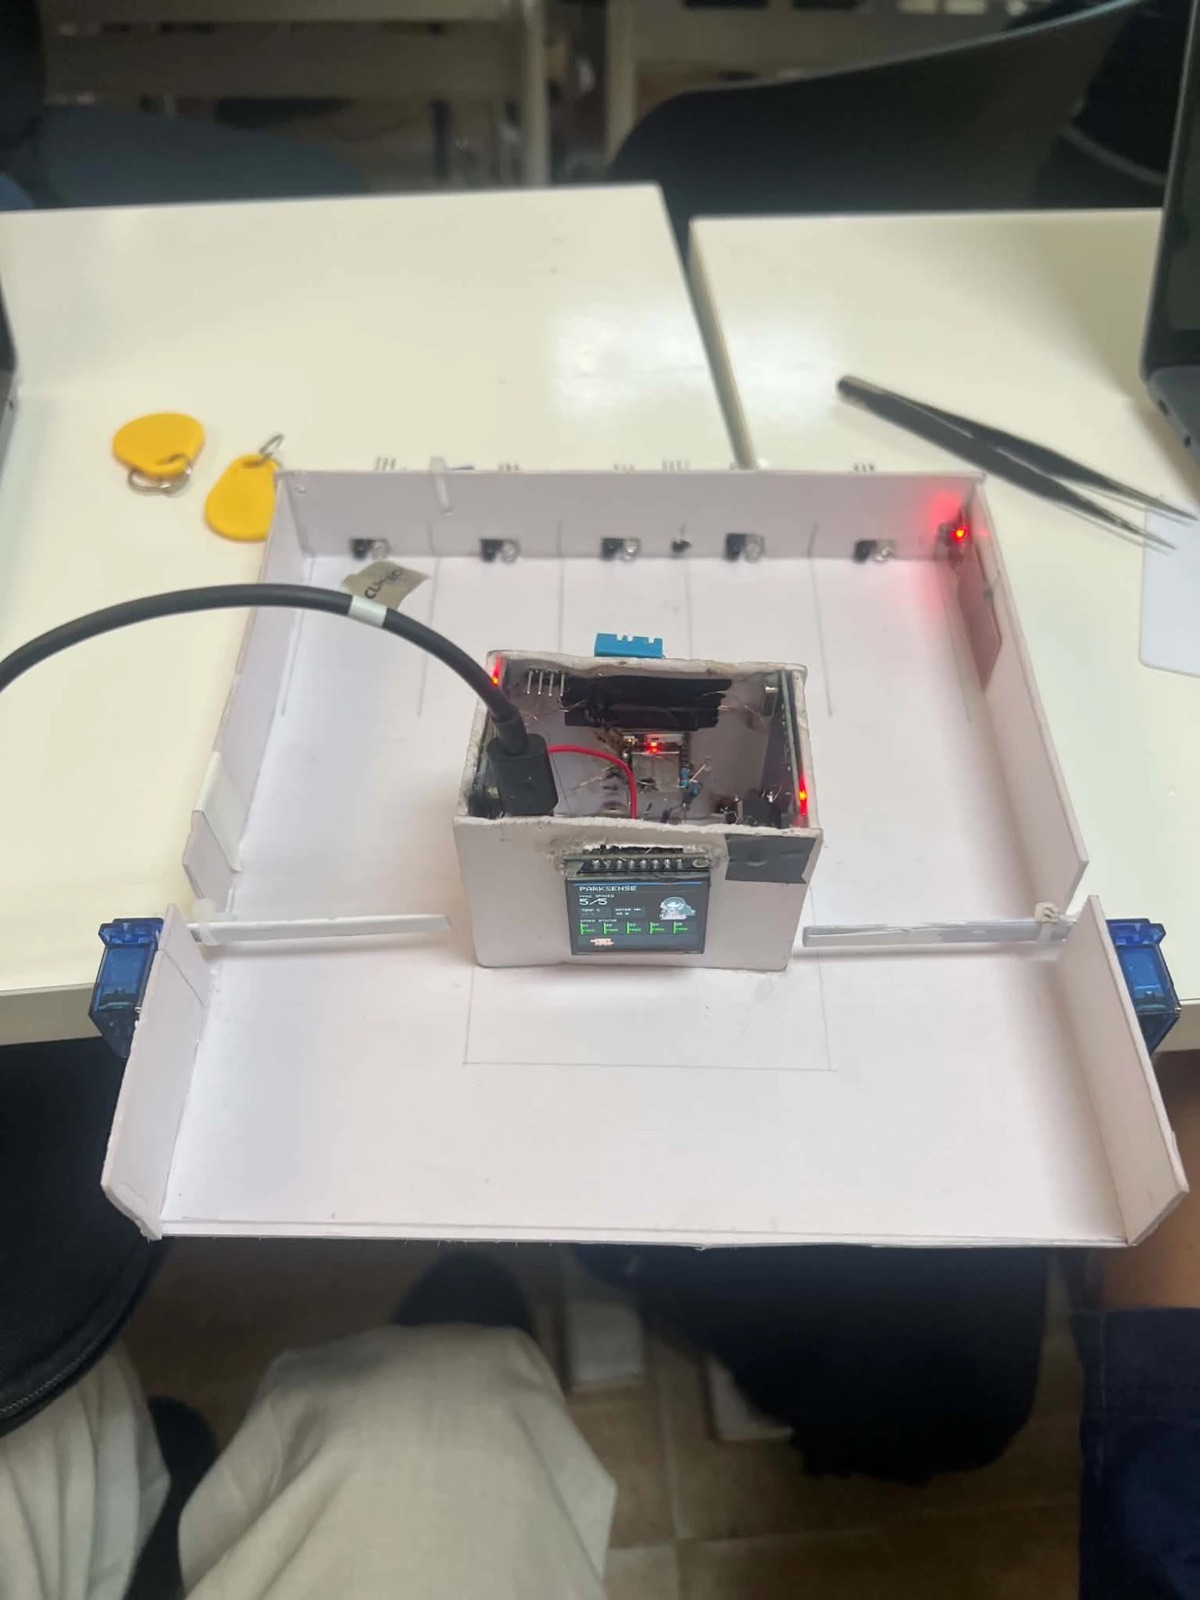
\includegraphics[width=\linewidth,height=0.36\textheight,keepaspectratio]{photos/model_top.jpg}
  \caption{Nhìn từ phía cổng: 5 ô đỗ, hộp điều khiển với TFT, hai thanh chắn servo}\label{fig:model-top}
\end{subfigure}\hfill
\begin{subfigure}[t]{0.49\linewidth}\centering
  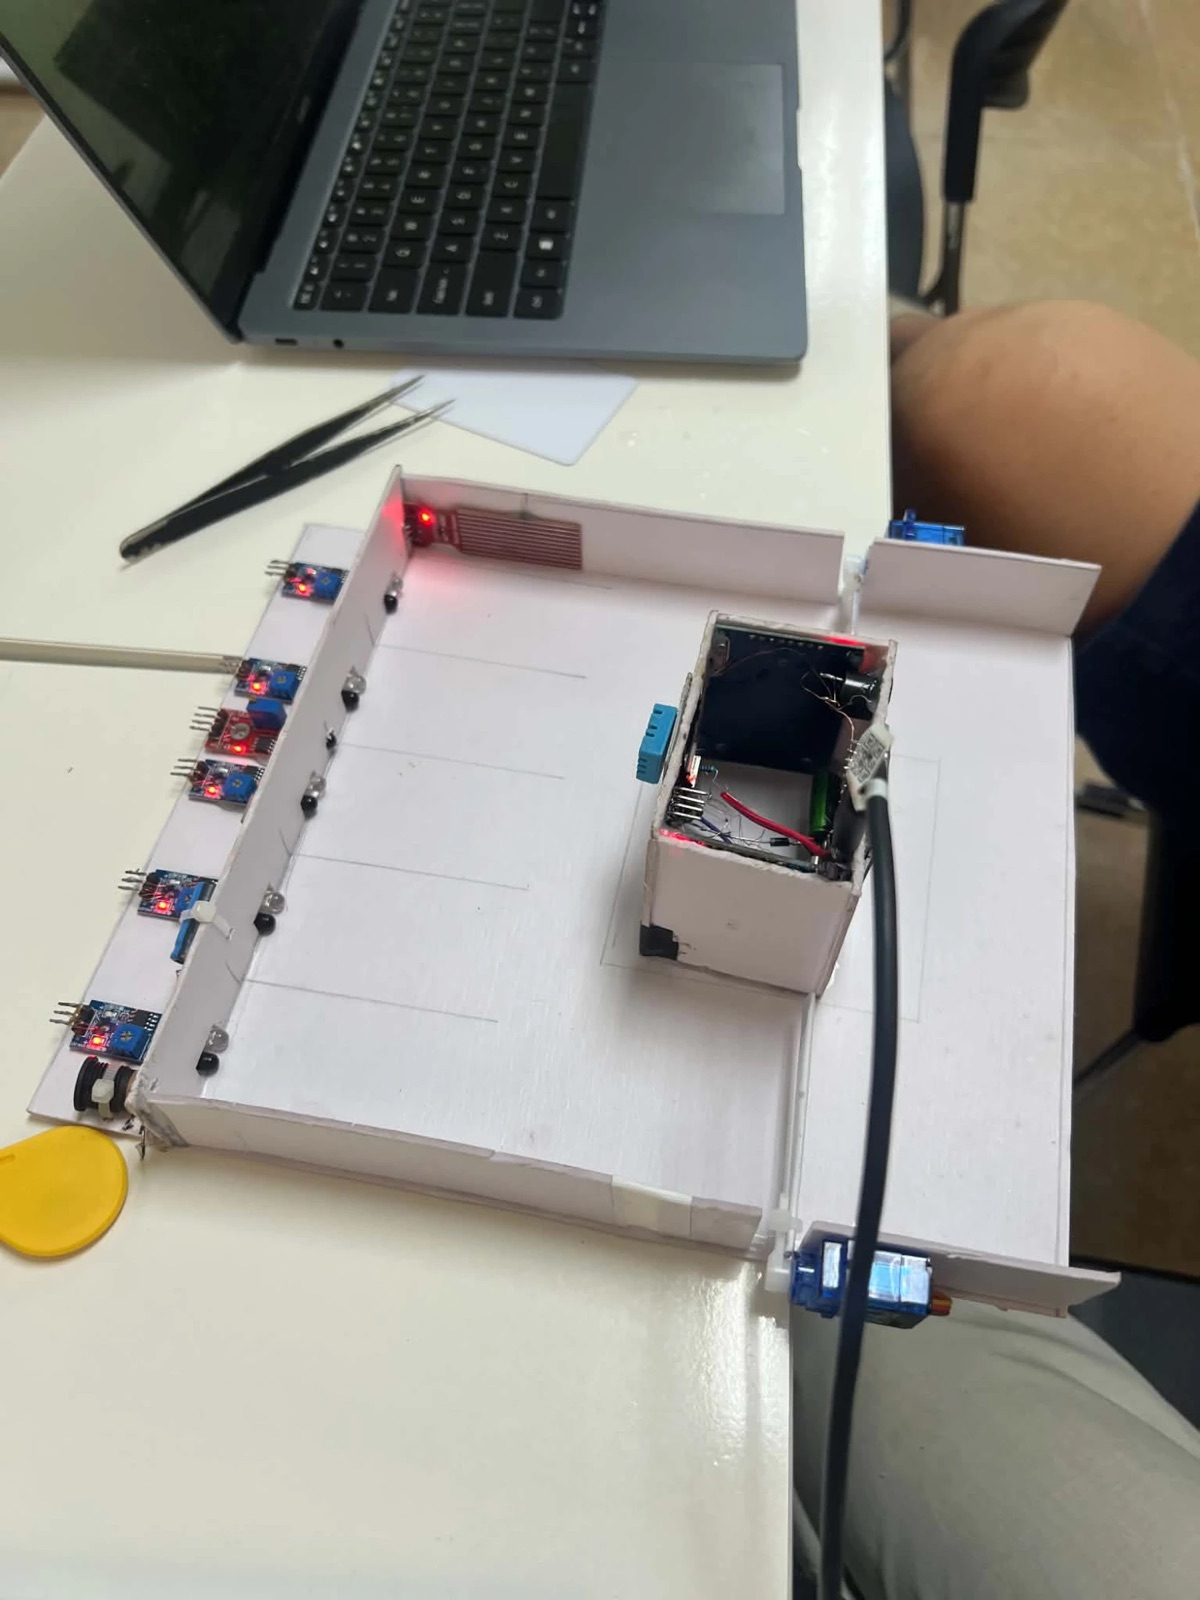
\includegraphics[width=\linewidth,height=0.36\textheight,keepaspectratio]{photos/model_angle.jpg}
  \caption{Góc nghiêng: dãy cảm biến ở mặt ngoài vách sau, cảm biến nước ở góc}\label{fig:model-angle}
\end{subfigure}

\vspace{4pt}
\begin{subfigure}[t]{0.49\linewidth}\centering
  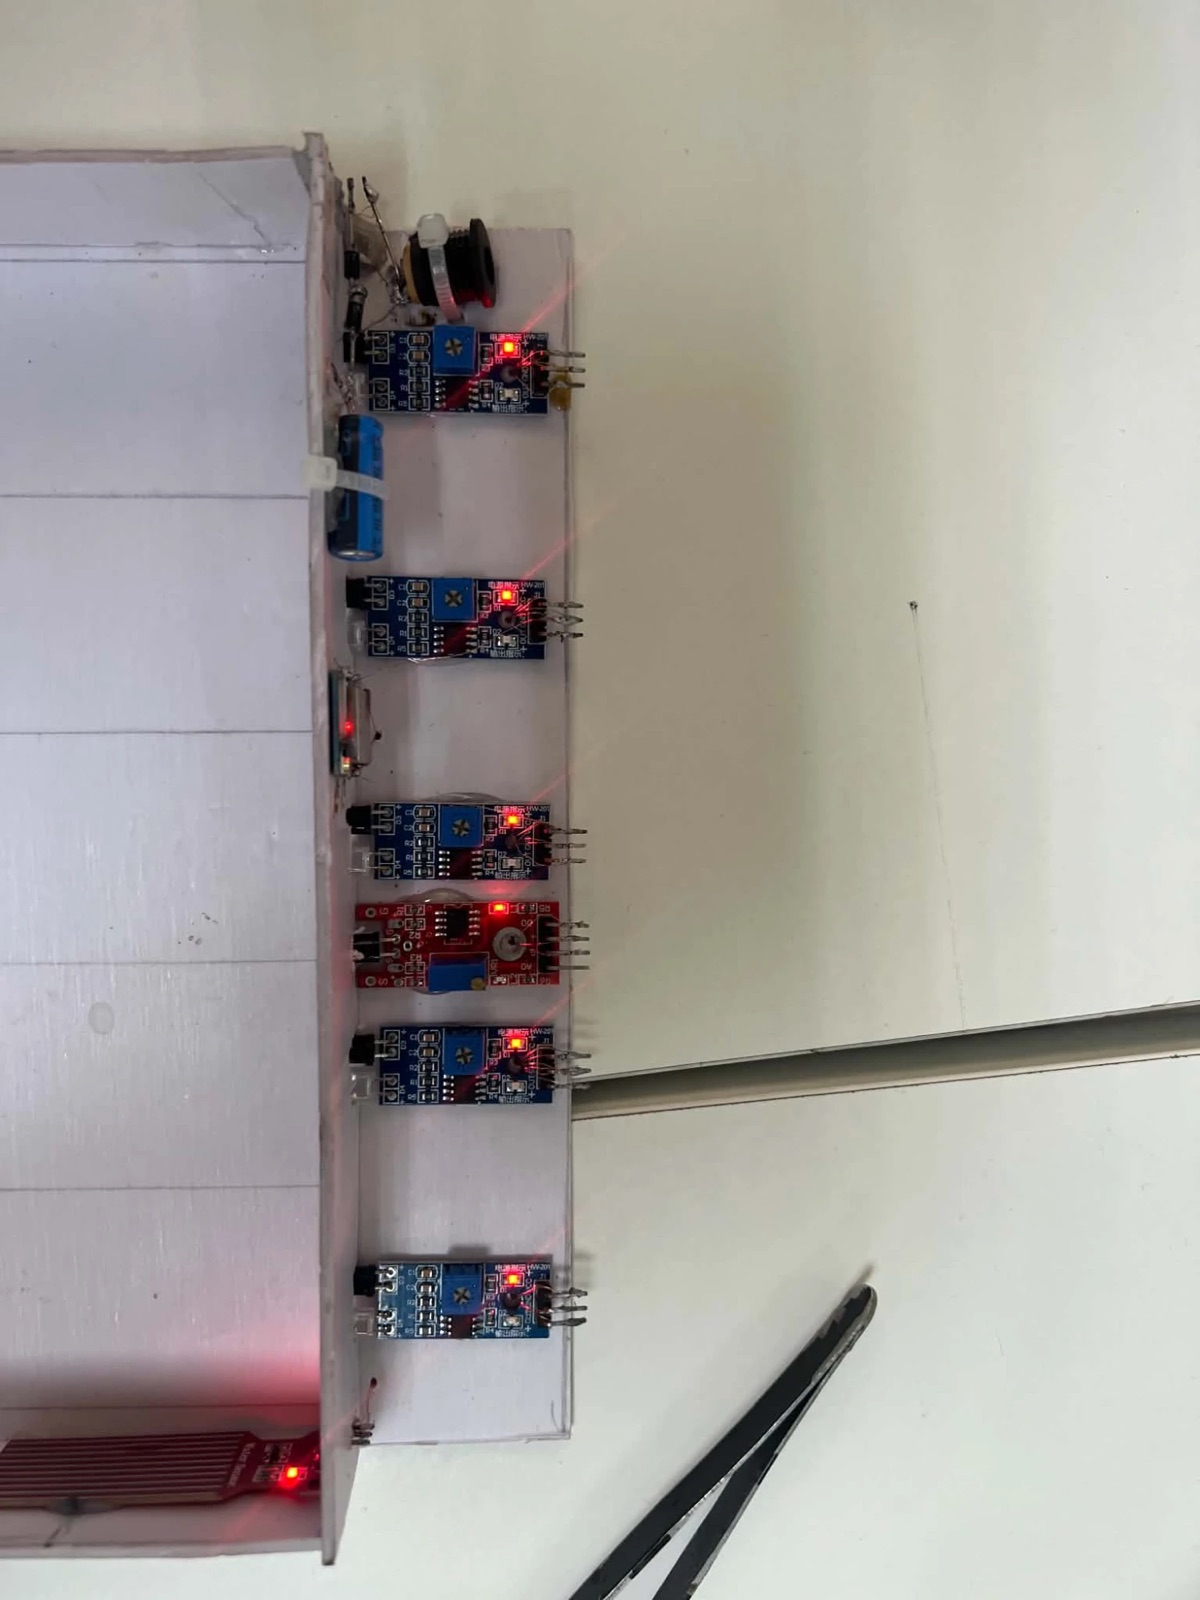
\includegraphics[width=\linewidth,height=0.36\textheight,keepaspectratio]{photos/model_sensorwall.jpg}
  \caption{Mặt ngoài vách sau: 5 module IR HW-201, module lửa (đỏ), jack nguồn DC, diode và tụ lọc}\label{fig:model-wall}
\end{subfigure}\hfill
\begin{subfigure}[t]{0.49\linewidth}\centering
  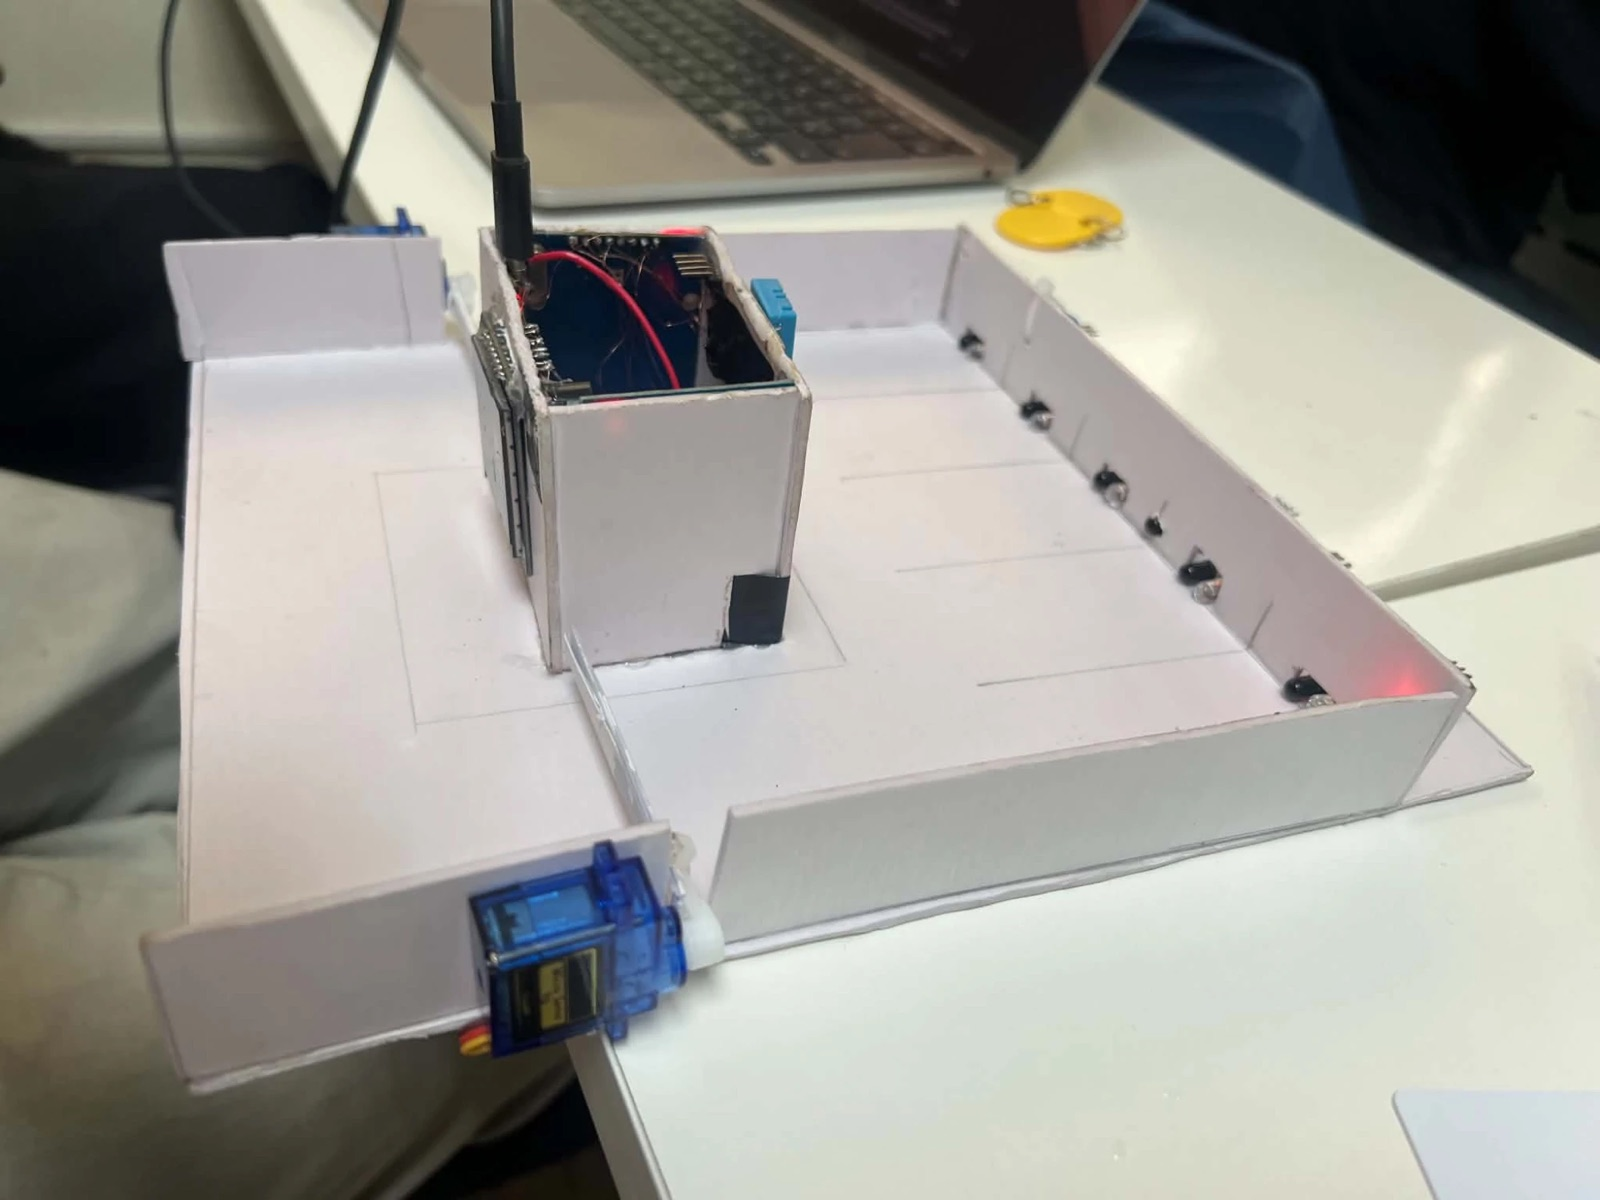
\includegraphics[width=\linewidth,height=0.36\textheight,keepaspectratio]{photos/model_gate.jpg}
  \caption{Cổng: servo SG90 gắn ở đầu vách, cần chắn quay ngang làn xe; DHT11 trên nóc hộp}\label{fig:model-gate}
\end{subfigure}
\caption{Mô hình bãi đỗ xe thông minh của nhóm}\label{fig:model}
\end{figure}

\begin{table}[H]
\centering\small
\caption{Vị trí lắp đặt từng thiết bị trên mô hình và lý do}\label{tab:placement}
\begin{tabularx}{\linewidth}{@{}p{3.1cm}p{4.3cm}X@{}}
\toprule
\textbf{Thiết bị} & \textbf{Vị trí} & \textbf{Lý do} \\ \midrule
5 module IR HW-201 & Mặt \emph{ngoài} vách sau, mỗi ô một module; LED phát/thu xuyên qua lỗ khoét vào đúng giữa ô & Dây và bo mạch nằm ngoài nên lòng bãi gọn, xe không vướng; khoảng cách tới đuôi xe chỉ vài cm, đúng tầm đo của IR. Mỗi module có biến trở chỉnh ngưỡng riêng theo độ phản xạ thực tế \\
Module lửa & Giữa dãy IR (giữa ô 3 và 4), đầu thu hướng vào lòng bãi & Góc nhìn $\approx$ 60° phủ được cả 5 ô từ vị trí trung tâm \\
Cảm biến mực nước & Góc trong của vách sau, sát sàn & Nước đọng tại điểm thấp và góc tường trước; đặt sát sàn để phát hiện sớm \\
Hộp điều khiển & Giữa bãi, giữa hai làn & Dây tới cảm biến, đầu đọc và servo đều ngắn; che bo mạch khỏi va chạm \\
TFT ST7789 & Mặt trước hộp, quay ra cổng & Người lái nhìn thấy số chỗ trống, hóa đơn và cảnh báo ngay khi tới cổng \\
2 đầu đọc RC522 & Hai hông hộp, mỗi đầu đọc quay ra một làn & Người lái quẹt thẻ từ trong xe ở đúng làn của mình; hai đầu đọc cách nhau cả hộp nên ít nhiễu chéo \\
2 servo SG90 & Đầu vách trái và phải, cần chắn quay ngang làn & Trục servo nằm ngoài làn, cần chắn nhẹ (nhựa) nên mô-men 1,8\,kg$\cdot$cm là dư \\
DHT11 & Nóc hộp điều khiển & Ra khỏi lòng hộp để không đo nhầm nhiệt do bo mạch tỏa ra \\
Jack DC, diode, tụ hóa & Mặt ngoài vách sau, cạnh dãy cảm biến & Một điểm cấp nguồn cho cả mô hình; xem đoạn ``Nguồn điện'' \\
\bottomrule
\end{tabularx}
\end{table}

\section{Sơ đồ chân}
\begin{table}[H]
\centering\small
\caption{Sơ đồ chân máy chủ ESP32-C3}\label{tab:pin-srv}
\begin{tabularx}{\linewidth}{@{}llX@{}}
\toprule
\textbf{Tín hiệu} & \textbf{GPIO} & \textbf{Ghi chú} \\ \midrule
TFT SCK / MOSI & 4 / 6 & SPI2 qua GPIO matrix; màn hình không cần MISO \\
TFT DC / RST / CS & 7 / 3 / 10 & Chọn lệnh–dữ liệu, reset, chọn chip \\
TFT đèn nền & 5 & Tắt khi khởi tạo để không thấy rác, bật sau khi sẵn sàng \\
Servo cổng vào / ra & 0 / 1 & Chân thường (bo không dùng thạch anh 32\,kHz) \\
Còi & 9 & Tích cực mức thấp; GPIO9 là chân strapping có kéo lên, trùng với trạng thái ``im lặng'' \\
\bottomrule
\end{tabularx}
\end{table}

\begin{table}[H]
\centering\small
\caption{Sơ đồ chân Sensor Client và RFID Client (ESP8266)}\label{tab:pin-clients}
\begin{tabularx}{\linewidth}{@{}llX@{}}
\toprule
\textbf{Tín hiệu} & \textbf{GPIO} & \textbf{Ghi chú} \\ \midrule
\multicolumn{3}{@{}l}{\itshape Sensor Client} \\
Ô đỗ S1–S5 & 16, 4, 14, 13, 12 & Tránh chân strapping (0, 2, 15) và UART (1, 3) \\
Cảm biến lửa (DO) & 5 & Module dùng trong nhóm cho mức cao khi có lửa \\
Mực nước & A0 & Chân ADC duy nhất của ESP8266 \\ \midrule
\multicolumn{3}{@{}l}{\itshape RFID Client} \\
SPI SCK / MOSI / MISO & 14 / 13 / 12 & SPI phần cứng, dùng chung cho 2 đầu đọc \\
SS đầu đọc cổng vào & 5 (D1) & Mỗi thiết bị SPI cần chân chọn chip riêng \\
SS đầu đọc cổng ra & 4 (D2) & \\
RST chung & 16 (D0) & Dùng chung để tiết kiệm chân \\
DHT11 & 2 (D4) & GPIO2 cần mức cao khi khởi động, DHT11 có điện trở kéo lên \\
\bottomrule
\end{tabularx}
\end{table}

\paragraph{Nguồn điện.} Mô hình có một điểm cấp nguồn là jack DC trên vách sau
(Hình~\ref{fig:model-wall}); khi trình diễn có thể cấp qua cáp USB vào hộp điều
khiển. Ba chi tiết được thêm sau khi đo thực tế:
\begin{itemize}[nosep]
  \item \textbf{Diode nối tiếp} ở đầu vào: cắm nhầm cực adapter thì diode chặn, không
        làm hỏng ba bo mạch và các module.
  \item \textbf{Tụ hóa lớn} song song nguồn 5\,V: servo SG90 kéo vài trăm mA lúc khởi
        động; tụ cấp dòng tức thời này nên điện áp không sụt làm ESP32-C3 hay ESP8266
        reset khi thanh chắn chuyển động.
  \item \textbf{Servo lấy nguồn 5\,V}, không lấy từ chân 3V3 của bo (bộ ổn áp trên bo
        chỉ cho vài trăm mA), và \textbf{nối chung GND} với ESP32-C3 để xung PWM có cùng
        mức tham chiếu.
\end{itemize}

\section{Thành phần phần mềm}
\begin{table}[H]
\centering\small
\caption{Thành phần phần mềm và vai trò}\label{tab:software}
\begin{tabularx}{\linewidth}{@{}p{3.6cm}p{2.3cm}X@{}}
\toprule
\textbf{Thành phần} & \textbf{Phiên bản} & \textbf{Vai trò} \\ \midrule
ESP-IDF & 6.1 & Framework chính thức cho ESP32-C3: driver, Wi-Fi, lwIP, HTTP server \\
FreeRTOS & đi kèm ESP-IDF & Hệ điều hành thời gian thực: tác vụ, ưu tiên, mutex, thông báo tác vụ \\
\code{esp\_lcd} + SPI master & ESP-IDF & Driver ST7789, truyền ảnh qua DMA \\
LEDC, \code{esp\_timer} & ESP-IDF & PWM servo; hẹn giờ đóng thanh chắn \\
\code{esp\_http\_server} & ESP-IDF & Phục vụ trang web và API JSON \\
\code{espressif/mdns} & 1.14.1 & Tên \code{parking.local} trong mạng cục bộ \\
Arduino core ESP8266 & 3.x & Nền tảng cho hai client \\
MFRC522, DHT sensor library & thư viện Arduino & Đọc RFID, đọc DHT11 \\
ArduinoOTA & đi kèm core & Nạp firmware client qua Wi-Fi \\
HTML/CSS/JavaScript & thuần & Trang web, không framework, không CDN \\
\bottomrule
\end{tabularx}
\end{table}

\section{Các module mã nguồn của máy chủ}
\begin{table}[H]
\centering\small
\caption{Module firmware máy chủ (\file{Server/main/})}\label{tab:modules}
\begin{tabularx}{\linewidth}{@{}p{4.3cm}rX@{}}
\toprule
\textbf{Tệp} & \textbf{Dòng} & \textbf{Trách nhiệm} \\ \midrule
\file{main.c} & 43 & Khởi tạo NVS, khôi phục phiên, màn hình, còi, servo, mạng theo thứ tự \\
\file{parking/parking\_state.c} & 65 & Trạng thái bãi dùng chung, đồng hồ bãi (critical section) \\
\file{parking/json\_scan.c} & 81 & Hàm đọc JSON dùng chung, không cấp phát động \\
\file{parking/parking\_update.c} & 108 & Kiểm tra bản tin \code{parking\_update} và \code{climate} \\
\file{parking/rfid\_session.c} & 314 & Bản tin RFID, phiên gửi xe, phí, hóa đơn, thông báo, nhật ký, chống lặp, đối chiếu IR, lưu/khôi phục, đặt giờ \\
\file{parking/packet\_auth.c} & 135 & Ký/kiểm tra gói UDP bằng SipHash-2-4, cửa sổ chống phát lại \\
\file{parking/parking\_persist.c} & 47 & Lưu/đọc phiên, nhật ký, đồng hồ trong NVS \\
\file{barrier/servo.c} & 230 & PWM servo, hẹn giờ tự đóng, chế độ cháy \\
\file{buzzer/buzzer.c} & 29 & Còi tích cực mức thấp \\
\file{display/lcd\_display.c} & 623 & Giao diện TFT, màn hình cháy, ảnh động \\
\file{display/*\_gif.c} & dữ liệu & Khung ảnh động đã nén LZSS \\
\file{network/wifi\_sta.c} & 134 & Kết nối Wi-Fi, tự kết nối lại \\
\file{network/network\_service.c} & 81 & Khởi động mạng, mDNS, cập nhật IP cho mDNS \\
\file{network/udp/udp\_server.c} & 196 & Kiểm tra chữ ký, điều phối bản tin UDP, gửi ACK \\
\file{network/http/http\_server.c} & 244 & 12 route HTTP, API JSON, kiểm tra mã PIN \\
\bottomrule
\end{tabularx}
\end{table}

% =====================================================================
\chapter{Cài đặt môi trường, hệ điều hành và phần mềm mô phỏng}\label{chap:caidat}
% =====================================================================

\section{Hệ điều hành đã chọn}
\subsection{Trên thiết bị: FreeRTOS cho máy chủ, vòng lặp Arduino cho client}
\begin{table}[H]
\centering\small
\caption{Hệ điều hành trên từng bo mạch}\label{tab:os}
\begin{tabularx}{\linewidth}{@{}lXX@{}}
\toprule
\textbf{Bo mạch} & \textbf{Hệ điều hành / mô hình chạy} & \textbf{Tính năng được dùng} \\ \midrule
ESP32-C3 (máy chủ) & FreeRTOS (bản Espressif, đi kèm ESP-IDF 6.1), tick 100\,Hz & Tác vụ có ưu tiên, mutex, critical section, thông báo tác vụ, hẹn giờ \code{esp\_timer} \\
ESP8266 (client) & Không dùng RTOS: một vòng lặp \code{loop()} không chặn trên Arduino core & Đếm thời gian bằng \code{millis()}, mọi việc chia nhỏ để Wi-Fi luôn được phục vụ \\
\bottomrule
\end{tabularx}
\end{table}

\begin{lydo}[Tại sao máy chủ cần RTOS còn client thì không]
Máy chủ có nhiều việc chạy song song với chu kỳ khác nhau: nhận UDP bất kỳ lúc nào,
phục vụ HTTP, vẽ màn hình, chạy ảnh động 10 khung/giây, đóng thanh chắn đúng giờ.
Viết tất cả trong một vòng lặp buộc phải chia nhỏ mọi việc bằng tay, và chỉ một thao
tác chậm (vẽ màn hình $\approx$ 23\,ms) cũng làm trễ việc khác. FreeRTOS cho phép mỗi
việc là một tác vụ có ưu tiên riêng: việc quan trọng (thanh chắn, nhận bản tin)
luôn chạy trước việc trang trí (ảnh động). Client chỉ làm tuần tự vài việc ngắn
(đọc cảm biến, gửi gói tin), một vòng lặp không chặn là đủ và đơn giản hơn.
\end{lydo}

\subsection{Trên máy phát triển}
Toàn bộ công cụ chạy trên \textbf{Windows 10/11, macOS hoặc Linux}. Nhóm đã phát
triển trên macOS và Windows. Các lệnh trong báo cáo dùng được trên cả ba hệ điều
hành, khác biệt duy nhất là tên cổng nối tiếp (Bảng~\ref{tab:ports}).

\section{Bản quyền phần mềm}
Mọi phần mềm dùng trong đề tài đều \textbf{miễn phí và mã nguồn mở}, nên không cần
bản dùng thử (trial) hay giấy phép trả phí:
\begin{table}[H]
\centering\small
\caption{Phần mềm cần cài và giấy phép}\label{tab:licenses}
\begin{tabularx}{\linewidth}{@{}lXl@{}}
\toprule
\textbf{Phần mềm} & \textbf{Dùng để} & \textbf{Giấy phép} \\ \midrule
ESP-IDF 6.1 (qua ESP-IDF Installation Manager) & Biên dịch, nạp firmware máy chủ & Apache 2.0 \\
Visual Studio Code + ESP-IDF extension (tùy chọn) & Soạn thảo, build/flash bằng giao diện & MIT / Apache 2.0 \\
Arduino IDE 2.x & Biên dịch, nạp hai client & AGPL-3.0 \\
Arduino core ESP8266 & Hỗ trợ bo ESP8266 & LGPL-2.1 \\
MFRC522, DHT sensor library & Thư viện thiết bị & Unlicense / MIT \\
Python 3 & Chạy công cụ giả lập client & PSF \\
Trình biên dịch C/C++ (clang hoặc gcc) & Chạy bộ kiểm thử trên máy tính & Apache 2.0 / GPL \\
Git & Lấy mã nguồn & GPL-2.0 \\
\bottomrule
\end{tabularx}
\end{table}

\section{Cài đặt từng phần mềm}
\subsection{ESP-IDF 6.1 (cho máy chủ)}
\begin{enumerate}
  \item Tải \textbf{ESP-IDF Installation Manager (EIM)} tại
        \url{https://dl.espressif.com/dl/eim/} và cài như ứng dụng thông thường.
  \item Mở EIM, chọn \textbf{ESP-IDF v6.1}, mục tiêu \textbf{esp32c3}, bấm cài đặt.
        EIM tự tải trình biên dịch RISC-V, Python và các công cụ.
  \item Mở terminal ESP-IDF. Windows: shortcut ``ESP-IDF 6.1 PowerShell'' do EIM tạo.
        macOS/Linux: nạp script kích hoạt do EIM tạo, ví dụ:
\begin{lstlisting}[style=shell]
source ~/.espressif/tools/activate_idf_v6.1.sh
\end{lstlisting}
  \item Kiểm tra: \code{idf.py --version} phải in \code{ESP-IDF v6.1}.
\end{enumerate}
ESP32-C3 SuperMini dùng USB Serial/JTAG tích hợp nên \textbf{không cần cài driver}.

\subsection{Arduino IDE và ESP8266 (cho hai client)}
\begin{enumerate}
  \item Cài Arduino IDE 2.x từ \url{https://www.arduino.cc/en/software}.
  \item \emph{File → Preferences → Additional boards manager URLs}, thêm:\\
        \url{https://arduino.esp8266.com/stable/package_esp8266com_index.json}
  \item \emph{Tools → Board → Boards Manager}, tìm \textbf{esp8266}, cài.
  \item \emph{Tools → Manage Libraries}, cài \textbf{MFRC522} (GithubCommunity) và
        \textbf{DHT sensor library} (Adafruit, chấp nhận cài kèm Adafruit Unified Sensor).
  \item Bo NodeMCU dùng chip USB-UART CH340 hoặc CP2102: nếu máy không nhận cổng,
        cài driver tương ứng của nhà sản xuất chip.
\end{enumerate}

\subsection{Công cụ cho giả lập và kiểm thử}
\begin{itemize}
  \item \textbf{Python 3.8+}: có sẵn trên macOS/Linux; Windows tải tại python.org. Không cần thư viện ngoài.
  \item \textbf{Trình biên dịch C/C++}: macOS \code{xcode-select --install}; Ubuntu
        \code{sudo apt install build-essential}; Windows dùng MSYS2/MinGW hoặc WSL.
\end{itemize}

\section{Phần mềm mô phỏng và các tính năng chính}
Đề tài dùng hai công cụ mô phỏng do nhóm tự viết, giúp phát triển và kiểm tra hệ
thống khi chưa có (hoặc không mang theo) đủ phần cứng.

\subsection{Bộ giả lập client bằng Python (\file{examples/})}
\begin{table}[H]
\centering\small
\caption{Công cụ giả lập client}\label{tab:simulators}
\begin{tabularx}{\linewidth}{@{}lX@{}}
\toprule
\textbf{Công cụ} & \textbf{Tính năng} \\ \midrule
\file{udp\_sender.py} & Giả lập Sensor Client: gửi một bản tin \code{parking\_update} (5 ô đỗ, mực nước, cháy) tới máy chủ thật qua UDP broadcast \\
\file{udp\_rfid\_sender.py} & Giả lập RFID Client: gửi \code{rfid\_event} với UID bất kỳ và cổng \code{--gate in|out}; chạy hai lần để giả lập vào rồi ra \\
\file{udp\_sender\_espidf.c} & Ví dụ gửi bản tin từ một bo ESP-IDF khác \\
\bottomrule
\end{tabularx}
\end{table}
Máy tính chỉ cần kết nối Wi-Fi \code{ESP32-Parking}; máy chủ không phân biệt bản tin
đến từ ESP8266 thật hay từ script, nên toàn bộ màn hình, thanh chắn, còi, trang web và
nhật ký đều được kiểm tra như thật.

\subsection{Mô phỏng phần cứng Arduino trên máy tính (\file{tests/arduino/})}
Đây là lớp giả lập các thư viện Arduino/ESP8266: đồng hồ \code{millis()} điều khiển
được, mức logic của từng chân, giá trị ADC, Wi-Fi bật/tắt, gói UDP được ghi lại,
đầu đọc RFID có thể ``đặt thẻ'' và DHT11 trả nhiệt độ tùy ý. Nhờ vậy \emph{chính mã
nguồn} \file{SensorClient.ino} và \file{RFIDClient.ino} được biên dịch và chạy trên
máy tính, mỗi bản tin chúng gửi được đưa thẳng vào bộ đọc JSON thật của máy chủ để
kiểm tra hai bên ``nói cùng một ngôn ngữ''. Chi tiết ở Chương~\ref{chap:kiemthu}.

\begin{lydo}[Tại sao tự viết công cụ mô phỏng thay vì dùng trình mô phỏng có sẵn]
Các trình mô phỏng vi điều khiển trực tuyến hỗ trợ ESP32-C3 nhưng không mô phỏng
được việc ba bo mạch nói chuyện với nhau qua Wi-Fi, và không có mô hình cho cả
MFRC522 lẫn module lửa/nước cụ thể của nhóm. Giả lập ở mức \emph{giao thức} (script
Python gửi bản tin thật) và ở mức \emph{thư viện} (đồng hồ, chân, UDP giả) kiểm tra
đúng phần logic nhóm tự viết, chạy trong vài giây, lặp lại được và không phụ thuộc
dịch vụ bên ngoài.
\end{lydo}

% =====================================================================
\chapter{Thiết kế và phân tích kiến trúc}\label{chap:thietke}
% =====================================================================

Chương này đi từ tổng thể đến chi tiết: kiến trúc triển khai và mạng
(\S\ref{sec:trienkhai}), kiến trúc phần mềm máy chủ (\S\ref{sec:phanlop}), mô hình
tác vụ và đồng bộ (\S\ref{sec:tacvu}), các luồng hoạt động (\S\ref{sec:luong}), máy
trạng thái (\S\ref{sec:fsm}), giao thức (\S\ref{sec:giaothuc}), thiết kế chi tiết
từng module (\S\ref{sec:chitiet}), phân tích chất lượng kiến trúc (\S\ref{sec:phantich})
và demo (\S\ref{sec:demo}).

% ---------------------------------------------------------------------
\section{Kiến trúc triển khai và mạng}\label{sec:trienkhai}
\begin{figure}[H]
\centering
\mmd[1][0.6]{deploy}
\caption{Kiến trúc triển khai: RFID Client làm điểm truy cập; máy chủ, Sensor Client và điện thoại là trạm Wi-Fi}\label{fig:deploy}
\end{figure}

Hình~\ref{fig:deploy} cho thấy cấu trúc mạng hình sao quanh RFID Client. Bảng~\ref{tab:netparams}
liệt kê thông số mạng. Hai client gửi tới địa chỉ \emph{broadcast} \code{192.168.4.255}
nên không cần biết IP máy chủ; người dùng truy cập bằng tên \code{parking.local}
nên cũng không cần biết IP.

\begin{table}[H]
\centering\small
\caption{Thông số mạng}\label{tab:netparams}
\begin{tabularx}{\linewidth}{@{}lX@{}}
\toprule
SSID / mật khẩu & \code{ESP32-Parking} / \code{12345678}, WPA2-PSK, kênh 1, tối đa 4 trạm \\
Điểm truy cập & RFID Client, \code{192.168.4.1/24}, cấp IP bằng DHCP \\
Máy chủ & Trạm Wi-Fi, IP do DHCP cấp, tên \code{parking.local}, dịch vụ \code{\_http.\_tcp} cổng 80 \\
UDP & Máy chủ nghe cổng 3333; client gửi tới \code{192.168.4.255:3333} \\
HTTP & Cổng 80: trang web, \code{/api/parking}, \code{/api/barrier}, \code{/api/rfid} \\
\bottomrule
\end{tabularx}
\end{table}

\begin{lydo}[Tại sao RFID Client làm điểm truy cập và máy chủ dùng mDNS]
Đặt điểm truy cập trên một bo ESP8266 giải phóng ESP32-C3 khỏi việc quản lý trạm
(bộ đệm cho từng trạm, DHCP server), dành RAM cho màn hình. Hệ thống vẫn hoạt động
độc lập, không cần router hay Internet. Đổi lại, IP máy chủ do DHCP cấp và có thể
thay đổi; mDNS giải quyết bằng một tên cố định \code{parking.local}. Máy chủ còn
\emph{chủ động thông báo lại} tên này mỗi khi nhận địa chỉ mới (sự kiện
\code{IP\_EVENT\_STA\_GOT\_IP}), kể cả khi DHCP đổi địa chỉ mà không mất kết nối, nên
các thiết bị khác không bao giờ giữ một IP cũ.
\end{lydo}

\subsection{Giao thức truyền: UDP broadcast}
\begin{table}[H]
\centering\small
\caption{So sánh giao thức truyền dữ liệu cảm biến}\label{tab:proto}
\begin{tabularx}{\linewidth}{@{}lXXX@{}}
\toprule
& \textbf{UDP} & \textbf{HTTP/TCP} & \textbf{MQTT} \\ \midrule
Thiết lập kết nối & Không & Bắt tay 3 bước & Cần broker \\
Overhead/bản tin & 8 byte & Vài trăm byte & 2+ byte trên TCP \\
Bộ nhớ máy chủ & 1 socket, đệm 256\,B & Socket + đệm mỗi kết nối & Thêm broker \\
Khi mất gói & Mất, bản tin sau bù lại & Tự truyền lại & Có QoS \\
\bottomrule
\end{tabularx}
\end{table}

\begin{lydo}
Sensor Client gửi \textbf{toàn bộ trạng thái} (không phải ``sự kiện thay đổi''), và
nhắc lại mỗi giây. Mất một gói chỉ làm trễ tối đa 1\,s, không làm sai trạng thái lâu
dài, nên độ tin cậy của TCP là không cần thiết, trong khi chi phí của nó (bắt tay,
socket, bộ đệm) đáng kể trên vi điều khiển. Gửi broadcast giúp client không cần biết
IP máy chủ và cho phép máy tính trong mạng ``nghe'' để gỡ lỗi. JSON được chọn vì đọc
được trong log và dễ sinh từ \code{snprintf}/Python; bản tin dài 70–110 byte, nằm
gọn trong một gói UDP.
\end{lydo}

% ---------------------------------------------------------------------
\section{Kiến trúc phần mềm máy chủ}\label{sec:phanlop}
Firmware máy chủ được tổ chức theo \textbf{kiến trúc phân lớp} (Hình~\ref{fig:layers}):
mỗi lớp chỉ gọi lớp dưới nó. Lớp \emph{nghiệp vụ} (\file{parking/}) không phụ thuộc
phần cứng nên chạy được cả trên máy tính để kiểm thử.

\begin{figure}[H]
\centering
\begin{tikzpicture}[
  lay/.style={draw,thick,rounded corners=2pt,minimum height=1.05cm,align=center,font=\small},
  mod/.style={draw,rounded corners=2pt,fill=white,font=\scriptsize,align=center,minimum height=0.62cm,inner sep=2pt}]
\def\W{14.6}
\node[lay,fill=boxE,minimum width=\W cm] (app) at (0,4.2) {};
\node[anchor=west,font=\small\bfseries] at (-7.2,4.2) {Ứng dụng};
\node[mod] at (0.9,4.2) {\texttt{main.c}: khởi động theo thứ tự, fail-fast};
\node[lay,fill=boxA,minimum width=\W cm,minimum height=1.35cm] (svc) at (0,2.75) {};
\node[anchor=west,font=\small\bfseries,align=left] at (-7.2,2.75) {Dịch vụ};
\node[mod,minimum width=2.1cm] at (-3.4,2.75) {\texttt{udp\_server}\\điều phối bản tin};
\node[mod,minimum width=2.1cm] at (-1.05,2.75) {\texttt{http\_server}\\web + API};
\node[mod,minimum width=2.1cm] at (1.3,2.75) {\texttt{lcd\_display}\\giao diện TFT};
\node[mod,minimum width=1.6cm] at (3.35,2.75) {\texttt{servo}\\thanh chắn};
\node[mod,minimum width=1.4cm] at (5.05,2.75) {\texttt{buzzer}};
\node[mod,minimum width=1.4cm] at (6.45,2.75) {\texttt{network}\\Wi-Fi, mDNS};
\node[lay,fill=boxB,minimum width=\W cm] (dom) at (0,1.2) {};
\node[anchor=west,font=\small\bfseries,align=left] at (-7.2,1.2) {Nghiệp vụ};
\node[mod] at (-2.6,1.2) {\texttt{parking\_state}\\trạng thái bãi};
\node[mod] at (0.2,1.2) {\texttt{json\_scan}, \texttt{parking\_update}\\kiểm tra bản tin};
\node[mod] at (3.6,1.2) {\texttt{rfid\_session}\\phiên, phí, nhật ký, thông báo};
\node[lay,fill=boxC,minimum width=\W cm] (drv) at (0,-0.3) {};
\node[anchor=west,font=\small\bfseries,align=left] at (-7.2,-0.3) {ESP-IDF};
\node[mod] at (-3.5,-0.3) {\code{esp\_lcd} · SPI DMA};
\node[mod] at (-1.0,-0.3) {LEDC · GPIO};
\node[mod] at (1.2,-0.3) {\code{esp\_timer}};
\node[mod] at (3.2,-0.3) {lwIP · HTTPD};
\node[mod] at (5.6,-0.3) {Wi-Fi · mDNS · NVS};
\node[lay,fill=boxD,minimum width=\W cm] (os) at (0,-1.6) {};
\node[anchor=west,font=\small\bfseries,align=left] at (-7.2,-1.6) {RTOS};
\node[mod] at (0.9,-1.6) {FreeRTOS: tác vụ, mutex, critical section, thông báo tác vụ};
\node[lay,fill=gray!15,minimum width=\W cm,minimum height=0.8cm] (hw) at (0,-2.8) {\textbf{Phần cứng}: ESP32-C3 — SPI2, LEDC, GPIO, Wi-Fi};
\end{tikzpicture}
\caption{Kiến trúc phân lớp của firmware máy chủ}\label{fig:layers}
\end{figure}

\subsection{Phụ thuộc giữa các module}
Hình~\ref{fig:deps} là đồ thị phụ thuộc: mũi tên từ A đến B nghĩa là A gọi B. Mọi
mũi tên đều đi xuống lớp thấp hơn, hoặc từ \file{udp\_server} sang các thiết bị cùng
lớp dịch vụ, nên không có vòng phụ thuộc.

\begin{figure}[H]
\centering
\mmd[0.95][0.6]{deps}
\caption{Đồ thị phụ thuộc giữa các module (tím: ứng dụng, xanh dương: dịch vụ, xanh lá: nghiệp vụ, cam: dữ liệu)}\label{fig:deps}
\end{figure}

\begin{lydo}[Tại sao phân lớp như vậy]
(1) \emph{Kiểm thử được}: \file{parking\_state}, \file{json\_scan}, \file{parking\_update},
\file{rfid\_session} chỉ cần hai macro critical section và hàm đọc đồng hồ — thay bằng
hai tệp header giả là chạy được trên máy tính. (2) \emph{Thay đổi cục bộ}: đổi màn hình
khác chỉ sửa \file{lcd\_display}; đổi giao thức mạng chỉ sửa \file{udp\_server}.
(3) \emph{Không vòng phụ thuộc} (Hình~\ref{fig:deps}): \file{udp\_server} là nơi duy
nhất ``điều phối'' — nhận bản tin, gọi nghiệp vụ, rồi ra lệnh cho servo, còi và đánh
thức màn hình.
\end{lydo}

% ---------------------------------------------------------------------
\section{Mô hình tác vụ và đồng bộ}\label{sec:tacvu}
\begin{table}[H]
\centering\small
\caption{Các tác vụ đang chạy trên máy chủ}\label{tab:tasks}
\begin{tabularx}{\linewidth}{@{}lccp{3.0cm}X@{}}
\toprule
\textbf{Tác vụ} & \textbf{Ưu tiên} & \textbf{Stack} & \textbf{Đánh thức bởi} & \textbf{Nhiệm vụ} \\ \midrule
\code{udp\_server} & 5 & 4096 B & gói UDP đến & Kiểm tra bản tin, cập nhật trạng thái, ra lệnh servo/còi/màn hình \\
\code{httpd} & 5 & 4096 B & request HTTP & Trang web, API \\
\code{esp\_timer} (hệ thống) & cao & 3584 B & hẹn giờ & Gọi hàm đóng thanh chắn khi hết 3\,s \\
\code{lcd\_display} & 4 & 4096 B & thông báo tác vụ / 1\,s / 120\,ms & Vẽ lại màn hình khi dữ liệu đổi \\
\code{lcd\_animation} & 3 & 3072 B & mỗi khung (100\,ms) & Ảnh động trang trí \\
\code{mdns} & 1 & 4096 B & gói mDNS & Trả lời \code{parking.local} \\
\bottomrule
\end{tabularx}
\end{table}

\begin{figure}[H]
\centering
\mmd[0.95][0.6]{tasks}
\caption{Tác vụ (xanh dương, kèm mức ưu tiên), tài nguyên dùng chung (xanh lá) và cơ chế bảo vệ; nét đứt đỏ: đánh thức tác vụ}\label{fig:tasks}
\end{figure}

Hệ thống dùng \textbf{ba cơ chế đồng bộ} cho ba loại tình huống khác nhau:
\begin{itemize}
\item \textbf{Critical section} (\code{portENTER\_CRITICAL}) cho \file{parking\_state} và
  \file{rfid\_session}: vùng bảo vệ chỉ là vài lệnh sao chép cấu trúc nhỏ (vài micro
  giây). Rẻ hơn mutex; người đọc luôn nhận một bản sao nhất quán.
\item \textbf{Mutex} cho servo và panel LCD: vùng bảo vệ dài hơn (gửi dữ liệu SPI,
  ghi thanh ghi LEDC) và có thể chờ; mutex không tắt ngắt, cho phép tác vụ khác chạy
  và có kế thừa ưu tiên chống đảo ưu tiên.
\item \textbf{Thông báo tác vụ} (\code{xTaskNotifyGive}/\code{ulTaskNotifyTake}) để
  \file{udp\_server} đánh thức \file{lcd\_display} ngay khi có dữ liệu mới — nhẹ hơn
  semaphore (không cấp phát đối tượng) và thay cho việc hỏi vòng 500\,ms trước đây.
\end{itemize}

\begin{lydo}[Tại sao đặt ưu tiên như vậy]
Ưu tiên phản ánh mức độ quan trọng với người dùng: nhận bản tin và điều khiển thanh
chắn (5) liên quan trực tiếp đến xe đang chờ ở cổng; màn hình thông tin (4) quan
trọng hơn ảnh động trang trí (3); mDNS (1) chỉ trả lời truy vấn tên, chậm vài mili
giây không ảnh hưởng. Khi CPU bận, ảnh động chậm đi chứ thông tin không bị trễ.
\end{lydo}

% ---------------------------------------------------------------------
\section{Luồng hoạt động}\label{sec:luong}
\subsection{Khởi động máy chủ}
\begin{figure}[H]
\centering
\mmd[1][0.72]{boot}
\caption{Trình tự khởi động máy chủ (\file{main.c})}\label{fig:boot}
\end{figure}

\begin{lydo}[Tại sao thứ tự khởi động như vậy]
\textbf{NVS trước tiên} vì Wi-Fi đọc dữ liệu hiệu chuẩn từ NVS. \textbf{Màn hình
trước Wi-Fi}: framebuffer cần một khối bộ nhớ \emph{liền mạch} 115\,KB có khả năng
DMA; Wi-Fi cấp phát nhiều khối nhỏ làm phân mảnh heap, nên phải lấy khối lớn trước.
\textbf{Còi và servo trước mạng}: đưa còi về im lặng và thanh chắn về vị trí đóng
trước khi có bất kỳ lệnh nào từ mạng. \textbf{Mạng sau cùng}: chỉ nhận lệnh khi mọi
thiết bị đã sẵn sàng. \code{ESP\_ERROR\_CHECK} áp dụng nguyên tắc \emph{fail-fast}:
lỗi khởi tạo dẫn tới khởi động lại thay vì chạy ở trạng thái nửa vời.
\end{lydo}

\subsection{Xử lý bản tin UDP trên máy chủ}
\begin{figure}[H]
\centering
\mmd[1][0.6]{udpflow}
\caption{Lưu đồ điều phối bản tin trong tác vụ \code{udp\_server}}\label{fig:udpflow}
\end{figure}
Nếu socket lỗi, tác vụ đóng socket, chờ 1\,s rồi tạo lại — tự phục hồi mà không cần
khởi động lại máy chủ. Khi không có gói, tác vụ ngủ trong \code{recvfrom()} và
\textbf{không tốn CPU}.

\subsection{Vòng lặp của hai client}
\begin{figure}[H]
\centering
\mmd[1][0.62]{clientloops}
\caption{Vòng lặp không chặn của Sensor Client và RFID Client}\label{fig:clientloops}
\end{figure}

\subsection{Xe vào và ra bằng thẻ RFID}
\begin{figure}[H]
\centering
\mmd[1][0.62]{seq_rfid}
\caption{Biểu đồ tuần tự gửi xe (trên) và lấy xe (dưới)}\label{fig:seq-rfid}
\end{figure}

\subsection{Phát hiện cháy}
\begin{figure}[H]
\centering
\mmd[1][0.6]{seq_fire}
\caption{Biểu đồ tuần tự cảnh báo cháy}\label{fig:seq-fire}
\end{figure}

\subsection{Trang web giám sát}
Trình duyệt tải trang một lần, sau đó gọi \code{GET /api/parking} mỗi 1\,s,
\code{GET /api/rfid} mỗi 2\,s và \code{GET /api/barrier} khi mở trang. Lệnh điều
khiển dùng \code{POST}; các nút bị khóa đến khi có phản hồi để tránh gửi trùng.

% ---------------------------------------------------------------------
\section{Máy trạng thái}\label{sec:fsm}
\begin{figure}[H]
\centering
\mmd[1][0.6]{fsm_card}
\caption{Máy trạng thái của một thẻ RFID}\label{fig:fsm-card}
\end{figure}

\begin{figure}[H]
\centering
\mmd[1][0.6]{fsm_gate}
\caption{Máy trạng thái của một thanh chắn}\label{fig:fsm-gate}
\end{figure}

\begin{figure}[H]
\centering
\mmd[1][0.6]{fsm_footer}
\caption{Trạng thái vùng chân màn hình (footer) TFT; khi có cháy, toàn màn hình chuyển sang màn hình cảnh báo}\label{fig:fsm-footer}
\end{figure}

% ---------------------------------------------------------------------
\section{Giao thức và giao diện lập trình}\label{sec:giaothuc}
\begin{lstlisting}[language=json,caption={Bản tin \code{parking\_update} (Sensor Client → máy chủ)}]
{"type":"parking_update","slots":[1,0,0,1,0],"water_mm":0.2,"fire":false}
\end{lstlisting}
\begin{lstlisting}[language=json,caption={Bản tin \code{rfid\_event} (RFID Client → máy chủ)}]
{"type":"rfid_event","card_id":"A1B2C3D4","gate":"in","temperature_c":28.0}
\end{lstlisting}
\begin{lstlisting}[language=json,caption={Bản tin \code{climate} (RFID Client → máy chủ, mỗi 5\,s)}]
{"type":"climate","temperature_c":28.0}
\end{lstlisting}

\paragraph{Ký gói tin.} Mỗi bản tin JSON ở trên được gửi trong một ``phong bì'' có chữ ký;
máy chủ trả lời mỗi \code{rfid\_event} bằng một gói \code{ACK} cũng được ký:
\begin{lstlisting}[language={},numbers=none,caption={Định dạng gói UDP (\file{packet\_auth.c})}]
<tag: 16 hex><seq: 8 hex><JSON>         tag = SipHash-2-4(khoa 16 byte, seq + JSON)
16af4b44ee606cdf1234abcd{"type":"climate","temperature_c":28.0}
<tag><seq>ACK                           may chu -> RFID Client, cung seq voi su kien
\end{lstlisting}
\begin{itemize}[nosep]
  \item \textbf{Chữ ký} chứng minh gói đến từ thiết bị biết khóa: đổi bất kỳ byte nào
        (kể cả \code{seq}) thì chữ ký sai và gói bị bỏ trước khi đọc JSON.
  \item \textbf{Số thứ tự} \code{seq} chỉ tăng, kể cả qua lần khởi động lại của client
        (client giữ trước từng khối 65\,536 số trong EEPROM, mỗi khối chỉ ghi flash một
        lần). Máy chủ giữ một \textbf{cửa sổ chống phát lại} 32 số cho mỗi loại bản tin
        (giống IPsec): số mới được xử lý, số đã thấy là bản gửi lại (chỉ trả ACK), số
        cũ hơn cửa sổ là gói bị ghi lại để phát lại và bị bỏ.
\end{itemize}

\begin{lydo}[Tại sao SipHash-2-4 thay vì HMAC-SHA256]
SipHash là hàm băm có khóa (PRF) thiết kế riêng cho thông điệp ngắn: một gói của nhóm
chỉ 70–130 byte. Chữ ký 64 bit đủ chống giả mạo trong bối cảnh này (kẻ tấn công phải
gửi trung bình $2^{63}$ gói để đoán trúng). Thuật toán chỉ khoảng 30 dòng C, giống hệt
trên ESP32-C3, ESP8266 và Python, nên cả ba nơi dùng chung một định dạng và bộ kiểm thử
kiểm tra được bằng vector chuẩn của tác giả. HMAC-SHA256 có sẵn trong mbedTLS (máy chủ)
và BearSSL (ESP8266) nhưng hai thư viện có API khác nhau, phải mô phỏng thêm trong bộ
kiểm thử, và chữ ký dài gấp bốn.
\end{lydo}

\begin{table}[H]
\centering\small
\caption{Đặc tả trường dữ liệu và ràng buộc kiểm tra trên máy chủ}\label{tab:fields}
\begin{tabularx}{\linewidth}{@{}llX@{}}
\toprule
\textbf{Trường} & \textbf{Kiểu} & \textbf{Ràng buộc} \\ \midrule
\code{type} & chuỗi & \code{"parking\_update"}, \code{"rfid\_event"} hoặc \code{"climate"} \\
\code{slots} & mảng & Đúng 5 phần tử, mỗi phần tử 0 (trống) hoặc 1 (có xe) \\
\code{water\_mm} & số & $0 \le x \le 10\,000$ \\
\code{fire} & boolean & Tùy chọn (client cũ có thể không gửi); không chấp nhận 0/1 \\
\code{card\_id} & chuỗi & 1–31 ký tự \code{[A-Za-z0-9\_-]}, chuẩn hóa thành chữ hoa \\
\code{gate} & chuỗi & \code{"in"} hoặc \code{"out"} (không phân biệt hoa thường) \\
\code{temperature\_c} & số & $-40 \le x \le 125$ \\
Chung & — & Khóa lạ, khóa lặp, dữ liệu thừa sau \code{\}}, chuỗi có ký tự thoát đều bị từ chối \\
\bottomrule
\end{tabularx}
\end{table}

\begin{table}[H]
\centering\small
\caption[API HTTP của máy chủ (12 route)]{API HTTP của máy chủ (12 route); mọi lệnh POST cần header \code{X-Parking-Key} đúng mã PIN, sai thì trả 401}\label{tab:api}
\begin{tabularx}{\linewidth}{@{}lp{4.4cm}X@{}}
\toprule
\textbf{PT} & \textbf{Đường dẫn} & \textbf{Kết quả} \\ \midrule
GET & \code{/}, \code{/style.css} & Trang web nhúng trong firmware \\
GET & \code{/api/parking} & \code{received}, \code{slots}, \code{free}, \code{total}, \code{temperature\_c}, \code{water\_mm}, \code{fire} \\
GET & \code{/api/barrier} & \code{\{"in\_open":bool,"out\_open":bool\}} \\
GET & \code{/api/rfid} & \code{now\_s}, \code{fee\_per\_hour}, \code{parked[]} (thẻ, giờ vào, phí tạm tính), \code{log[]} (10 sự kiện mới nhất) \\
POST & \code{/api/barrier/}\allowbreak\code{<cổng>/<lệnh>} & Cổng \code{in}, \code{out}, \code{all}; lệnh \code{open}, \code{close}. Lỗi 500 nếu bị từ chối (ví dụ đóng khi có cháy) \\
POST & \code{/api/time} & Thân là giờ Unix (giây) từ trình duyệt; máy chủ đặt đồng hồ bãi và lưu NVS \\
\bottomrule
\end{tabularx}
\end{table}

% ---------------------------------------------------------------------
\section{Thiết kế chi tiết từng thành phần}\label{sec:chitiet}

\subsection{Thanh chắn: PWM phần cứng và hẹn giờ một lần}
Servo SG90 nhận xung chu kỳ 20\,ms; độ rộng xung quyết định góc (Hình~\ref{fig:pwm}).
\begin{figure}[H]
\centering
\begin{tikzpicture}[x=0.55cm,y=0.7cm,font=\scriptsize]
\draw[-{Stealth}] (0,0) -- (23,0) node[right]{$t$ (ms)};
\draw[-{Stealth}] (0,0) -- (0,1.8) node[left]{PWM};
\draw[thick,accent] (0,0) -- (0,1.2) -- (1.45,1.2) -- (1.45,0) -- (20,0) -- (20,1.2) -- (21.45,1.2) -- (21.45,0) -- (22.5,0);
\draw[{Stealth}-{Stealth}] (0,-0.5) -- node[below]{chu kỳ $T = 20$\,ms (50\,Hz)} (20,-0.5);
\draw[{Stealth}-{Stealth}] (0,1.5) -- node[above]{$p$} (1.45,1.5);
\node[align=left,anchor=west] at (3,1.0) {$p = 500$\,µs $\to 0°$\quad $p = 1450$\,µs $\to 90°$\quad $p = 2400$\,µs $\to 180°$};
\end{tikzpicture}
\caption{Dạng xung điều khiển servo SG90}\label{fig:pwm}
\end{figure}
\begin{equation}
  p(\theta) = 500 + \frac{1900\,\theta}{180}\ \text{µs}, \qquad
  D = \left\lfloor \frac{p \cdot (2^{14}-1)}{20\,000} \right\rfloor
\end{equation}
Với $\theta=90°$: $p=1450$\,µs, $D=1187$; với $\theta=0°$: $p=500$\,µs, $D=409$.

\begin{lydo}[Tại sao 50\,Hz, 14 bit, LEDC]
\textbf{50\,Hz} là tần số chuẩn của servo RC analog. \textbf{14 bit} là độ phân giải
lớn nhất của LEDC trên ESP32-C3: mỗi bước $20\,000/16\,384 \approx 1{,}22$\,µs $\approx 0{,}12°$,
mịn hơn nhiều vùng chết $\approx$1° của SG90 nên servo không rung. \textbf{LEDC} là PWM
phần cứng: xung phát liên tục mà CPU không can thiệp, servo giữ góc ổn định dù
Wi-Fi hay màn hình đang bận. Dải 500–2400\,µs là giá trị đo thực tế của SG90 (danh
nghĩa 1000–2000\,µs không đủ 180°).
\end{lydo}

\begin{lydo}[Tại sao dùng hẹn giờ một lần (\code{esp\_timer}) thay vì tác vụ hỏi vòng]
Phiên bản đầu dùng một tác vụ thức dậy 20 lần/giây để kiểm tra hạn đóng. Phiên bản
hiện tại tạo một \code{esp\_timer} một lần cho mỗi cổng: hàm đóng được gọi \emph{đúng}
lúc hết 3\,s (sai số micro giây thay vì 50\,ms), CPU không bị đánh thức vô ích và tiết
kiệm 3\,KB stack. Vì một lệnh khác có thể ``đua'' với hàm đóng, hàm đóng kiểm tra lại
hạn đóng dưới mutex; lệnh tay từ web đặt hạn về 0 và dừng hẹn giờ — \textbf{lệnh của
người vận hành luôn thắng}.
\end{lydo}

Hai cổng được mô tả bằng cùng một cấu trúc (kênh LEDC, chân, hướng lắp, trạng thái,
hạn đóng, hẹn giờ) nên một hàm xử lý cho cả hai. Thanh chắn ra lắp đối xứng nên góc
mở/đóng đảo ngược (0° mở, 90° đóng) — chỉ khai báo ở một hàm. Cả hai cổng \textbf{luôn
khởi động ở vị trí đóng}, nên trạng thái không cần lưu vào flash; phiên bản trước ghi
NVS mỗi lần thanh chắn chuyển động đã được bỏ (chậm và làm mòn flash vô ích).

\subsection{Màn hình: SPI DMA, vẽ theo sự kiện, ảnh động tiền xử lý}
\begin{lydo}[Tại sao SPI 40\,MHz và DMA]
Một khung hình đầy đủ là $240\times240\times16 = 921\,600$ bit; ở 40\,MHz mất
$\approx$ 23\,ms, tối đa $\approx$ 43 khung/giây — dư cho giao diện tĩnh và màn hình cháy
8 khung/giây. 40\,MHz bằng đúng $80\,\text{MHz}/2$ (không sai số chia tần) và dưới giới
hạn ghi $\approx$ 62\,MHz của ST7789, chừa biên an toàn cho dây cắm. DMA cho phép CPU
làm việc khác trong lúc ảnh được đẩy ra.
\end{lydo}

\begin{itemize}
\item \textbf{Framebuffer RGB565} 115\,200 byte: toàn bộ giao diện được vẽ vào RAM rồi gửi
  một lần. Màu được lưu sẵn theo thứ tự byte của ST7789 (byte cao trước) vì
  ESP32-C3 là little-endian.
\item \textbf{Hàm tô hình chữ nhật} cắt biên một lần và tô từng dòng liên tục thay vì
  kiểm tra biên và đảo byte cho từng điểm ảnh.
\item \textbf{Font 5$\times$7 tự định nghĩa} cho A–Z, 0–9 (180 byte) — không cần thư viện
  đồ họa lớn như LVGL cho một giao diện cố định.
\item \textbf{Vẽ theo sự kiện}: \file{udp\_server} đánh thức tác vụ màn hình bằng thông
  báo tác vụ ngay khi có dữ liệu; nếu không có gì, tác vụ chỉ thức mỗi 1\,s (để hết hạn
  hóa đơn/thông báo) hoặc 120\,ms khi có cháy (để lửa nhấp nháy). Màn hình chỉ vẽ lại
  khi nội dung thực sự thay đổi.
\end{itemize}

\begin{table}[H]
\centering\small
\caption{Dữ liệu ảnh động sau tiền xử lý và nén LZSS}\label{tab:lzss}
\begin{tabular}{@{}lrrrr@{}}
\toprule
\textbf{Ảnh} & \textbf{Kích thước} & \textbf{Số khung} & \textbf{Dữ liệu thô} & \textbf{Sau nén} \\ \midrule
Kaoruko & 96$\times$96 & 10 & 184\,320 B & 70\,564 B (2,6$\times$) \\
Claude & 68$\times$46 & 18 & 112\,608 B & 16\,204 B (6,9$\times$) \\
\bottomrule
\end{tabular}
\end{table}

\begin{lydo}[Tại sao tiền xử lý ảnh trên máy tính]
Ảnh gốc có nền trắng cần xóa và điểm ảnh cần đảo byte. Phiên bản trước làm việc
này trên chip cho \emph{mọi khung hình}, 10 lần/giây: thuật toán loang tìm nền trắng
nối với viền (cần thêm 1,2\,KB RAM) rồi đảo byte 9\,216 điểm. Vì ảnh không bao giờ
đổi, nhóm làm một lần trên máy tính và lưu kết quả đã xử lý: firmware chỉ còn giải
nén. Kết quả được kiểm chứng giống từng điểm ảnh với cách cũ trên cả 28 khung, dữ
liệu còn nhỏ hơn (86\,768 so với 87\,977 byte). LZSS có bộ giải nén $\approx$ 40 dòng,
không cần bộ nhớ phụ và kiểm tra biên đầy đủ nên dữ liệu hỏng không gây ghi tràn.
\end{lydo}

\textbf{Hai bộ đệm DMA} (2 $\times$ 18\,432 byte) được dùng luân phiên cho ảnh động:
lệnh vẽ chỉ \emph{xếp hàng} giao dịch DMA rồi trả về, nên giải nén khung kế tiếp vào
cùng bộ đệm khi DMA chưa đọc xong sẽ làm hình bị xé. Hai tác vụ cùng vẽ lên một
panel nên dùng chung một mutex.

\subsection{Bộ kiểm tra bản tin JSON}
\begin{lydo}[Tại sao tự viết thay vì dùng thư viện cJSON]
Gói UDP là \emph{ranh giới tin cậy}: bất kỳ thiết bị nào trong mạng đều gửi được.
cJSON cấp phát heap cho từng nút (phân mảnh heap khi chạy lâu) và chấp nhận mọi JSON
hợp lệ. Bộ đọc tự viết (\file{json\_scan.c}, 81 dòng, dùng chung cho cả hai loại bản
tin) \textbf{không cấp phát động}, chỉ chấp nhận đúng lược đồ (Bảng~\ref{tab:fields})
và có \textbf{vòng lặp giới hạn} (tối đa 4 khóa) nên thời gian xử lý bị chặn trên.
Bộ đệm nhận 256 byte, đọc tối đa 255 byte và luôn kết thúc bằng \code{'\textbackslash0'}.
\end{lydo}

\subsection{Phiên gửi xe, phí, thông báo và nhật ký}
\begin{itemize}
\item \textbf{Phiên}: mảng tĩnh 5 phần tử — bằng số chỗ đỗ, không có nhiều xe hơn số chỗ.
  Thời điểm vào lấy từ \code{esp\_timer\_get\_time()} (64 bit, micro giây, không tràn trong
  hơn 290\,000 năm).
\item \textbf{Phí}: $h=\max(1,\lceil t/3600\rceil)$, phí $=5000\,h$ VNĐ, tính bằng số
  nguyên \code{(t + 3599) / 3600}, bão hòa ở \code{UINT32\_MAX} nếu tràn.
\item \textbf{Thông báo từ chối} (sai cổng, bãi đầy): giữ 5\,s; lần quẹt hợp lệ tiếp
  theo xóa thông báo ngay.
\item \textbf{Nhật ký}: bộ đệm vòng 10 sự kiện ($\approx$ 520 byte), đọc ra theo thứ tự mới
  nhất trước; không dùng heap.
\end{itemize}

\begin{lydo}[Tại sao chọn các thông số này]
\textbf{5.000\,VNĐ/giờ, làm tròn lên, tối thiểu 1 giờ} là cách tính phổ biến của bãi
xe, dễ giải thích. \textbf{Hóa đơn 60\,s} đủ để tài xế đọc và trả tiền; \textbf{thông
báo 5\,s} đủ đọc mà không che hóa đơn quá lâu. \textbf{Thanh chắn mở 3\,s} đủ cho xe mô
hình đi qua nhưng không đủ để xe sau ``đi ké''. \textbf{Nhật ký 10 sự kiện} vừa một màn
hình điện thoại và tốn dưới 1\,KB RAM.
\end{lydo}

\subsection{Sensor Client: lọc nhiễu và gửi theo thay đổi}
\begin{figure}[H]
\centering
\begin{tikzpicture}[x=0.9cm,y=0.6cm,font=\scriptsize]
\node[anchor=east] at (-0.2,2.5) {Tín hiệu thô};
\draw[thick] (0,2) -- (2,2) -- (2,3) -- (2.3,3) -- (2.3,2) -- (2.5,2) -- (2.5,3) -- (2.7,3) -- (2.7,2) -- (2.9,2) -- (2.9,3) -- (11,3);
\node[anchor=east] at (-0.2,0.5) {Trạng thái};
\draw[thick,accent] (0,0) -- (3.9,0) -- (3.9,1) -- (11,1);
\draw[dashed,gray] (2.9,3.3) -- (2.9,-0.4);
\draw[dashed,gray] (3.9,3.3) -- (3.9,-0.4);
\draw[{Stealth}-{Stealth}] (2.9,-0.6) -- node[below]{ổn định 50\,ms} (3.9,-0.6);
\node[align=center] at (2.45,3.8) {nhiễu khi xe\\đang lăn vào};
\node[draw,fill=boxB,align=center] at (7.5,-0.9) {gửi \code{parking\_update} ngay};
\draw[-{Stealth},thick] (3.9,1) to[bend right=10] (6.2,-0.6);
\end{tikzpicture}
\caption{Chống rung: chỉ chấp nhận mức mới khi giữ ổn định 50\,ms, rồi gửi ngay}\label{fig:debounce}
\end{figure}

\begin{lydo}[Tại sao lọc 50\,ms và gửi theo thay đổi kèm nhắc lại 1\,s]
Mép xe và bánh xe làm tín hiệu IR bật/tắt liên tục trong vài chục mili giây khi xe
đang vào chỗ. Nhóm tinh chỉnh thực nghiệm từ 250\,ms xuống \textbf{50\,ms}: đủ lọc nhiễu
mà cảm giác tức thời. Trước đây trạng thái chỉ được gửi theo chu kỳ 1\,s nên thay đổi
có thể trễ đến 1\,s; nay \textbf{gửi ngay khi có thay đổi}, đồng thời vẫn \textbf{nhắc
lại mỗi giây} để một gói bị mất được sửa ở lần sau. Mỗi cảm biến có bộ đếm riêng.
\end{lydo}

Mực nước được quy đổi tuyến tính từ ADC 10 bit:
\begin{equation}
  h_{\text{mm}} =
  \begin{cases}
  0, & raw \le 20 \\[2pt]
  \dfrac{\min(raw, 700) - 20}{700 - 20} \cdot 40, & raw > 20
  \end{cases}
\end{equation}
trong đó 20 là mức nhiễu khi khô, 700 là giá trị khi ngập hoàn toàn và 40\,mm là
chiều dài vùng đo; ADC được đọc mỗi 250\,ms vì đọc quá dày ảnh hưởng Wi-Fi trên
ESP8266 trong khi mực nước thay đổi chậm.

\subsection{RFID Client: hai đầu đọc trên một bus SPI}
\begin{lydo}[Tại sao bật ăng-ten luân phiên, chờ 4\,ms, gain 48\,dB, chống lặp 2\,s]
Hai đầu đọc 13,56\,MHz đặt gần nhau sẽ \textbf{nhiễu chéo}; chỉ bật một ăng-ten tại
một thời điểm loại bỏ hoàn toàn vấn đề. Thẻ thụ động cần vài mili giây để nhận đủ năng
lượng: \textbf{4\,ms} đủ cho thẻ MIFARE mà chu kỳ quét vẫn ngắn. \textbf{Gain 48\,dB} bù
tầm đọc khi đầu đọc nằm sau vỏ mô hình. Thẻ để yên sẽ bị đọc liên tục; \textbf{chống
lặp 2\,s} áp dụng cho cả hai đầu đọc, tránh một lần quẹt bị gửi nhiều lần làm ``vào''
biến thành ``ra''. UID được đổi sang chuỗi hex bằng \textbf{bộ đệm cố định} thay vì
\code{String} của Arduino: không cấp phát heap mỗi lần quẹt, nên heap 80\,KB của
ESP8266 không bị phân mảnh khi chạy lâu. DHT11 đọc mỗi \textbf{5\,s} vì cảm biến cần ít
nhất 1\,s giữa hai lần đọc và nhiệt độ thay đổi chậm.
\end{lydo}

\subsection{Trang web}
\begin{lydo}[Tại sao hỏi vòng 1–2\,s thay vì WebSocket]
Hỏi vòng không giữ trạng thái kết nối trên máy chủ: mỗi request độc lập, xử lý xong
giải phóng ngay — phù hợp giới hạn socket và RAM, và đơn giản khi nhiều trình duyệt
cùng xem. Với dữ liệu thay đổi theo giây, độ trễ thêm tối đa 1\,s là chấp nhận được.
Trang web là HTML/CSS/JavaScript thuần, nhúng trong firmware bằng
\code{EMBED\_TXTFILES}: không cần phân vùng tệp, không phụ thuộc CDN (điện thoại kết nối
hotspot không có Internet).
\end{lydo}

% ---------------------------------------------------------------------
\section{Phân tích kiến trúc}\label{sec:phantich}
\subsection{Hiệu năng và độ trễ}
\begin{table}[H]
\centering\small
\caption{Ngân sách độ trễ của các luồng chính (ước tính từ thông số thiết kế)}\label{tab:latency}
\begin{tabularx}{\linewidth}{@{}lXr@{}}
\toprule
\textbf{Luồng} & \textbf{Thành phần} & \textbf{Tổng} \\ \midrule
Xe vào ô → màn hình TFT & lọc 50\,ms + gửi ngay + UDP vài ms + đánh thức + vẽ 23\,ms & $\approx$ 0,1\,s \\
Xe vào ô → trang web & như trên + hỏi vòng tối đa 1\,s & $\le$ 1,1\,s \\
Quẹt thẻ → thanh chắn mở & quét 2 đầu đọc $\approx$ 10\,ms + UDP + xử lý $<$ 1\,ms + servo 90° $\approx$ 0,15\,s & $\approx$ 0,2\,s \\
Có lửa → còi kêu & lọc 50\,ms + gửi ngay + UDP & $\approx$ 0,06\,s \\
Mất một gói \code{parking\_update} & sửa ở lần nhắc lại & $\le$ 1\,s \\
Mất một gói \code{rfid\_event} & gửi lại sau 300\,ms chờ ACK & $\approx$ 0,5\,s \\
\bottomrule
\end{tabularx}
\end{table}

\subsection{Bộ nhớ}
\begin{table}[H]
\centering\small
\caption{Sử dụng bộ nhớ của firmware máy chủ (đo bằng \code{idf.py size})}\label{tab:memory}
\begin{tabularx}{\linewidth}{@{}Xr@{}}
\toprule
\textbf{Hạng mục} & \textbf{Kích thước} \\ \midrule
DRAM tĩnh dùng / tổng (mã IRAM 81\,444 + \code{.data} 13\,792 + \code{.bss} 21\,504) & 116\,740 / 321\,296 B (36,3\%) \\
Framebuffer màn hình (heap, DMA) & 115\,200 B \\
2 bộ đệm ảnh động (heap, DMA) & 36\,864 B \\
Stack các tác vụ của ứng dụng & $\approx$ 19\,KB \\
Bảng phiên, hóa đơn, thông báo, nhật ký, cửa sổ chống phát lại & $<$ 1\,KB \\ \midrule
Ảnh firmware & 1\,092\,768 B \\
Phân vùng ứng dụng (\code{factory}) & 1\,536\,000 B (dùng 71,1\%) \\
\bottomrule
\end{tabularx}
\end{table}

\begin{lydo}[Tại sao phân vùng ứng dụng 1,5\,MB]
Bảng phân vùng mặc định chỉ có 1\,MB cho ứng dụng và đã đầy 98\% trước khi thêm mDNS.
Flash 2\,MB đủ chỗ cho phân vùng 1,5\,MB có sẵn trong ESP-IDF
(\code{partitions\_singleapp\_large.csv}), được khai báo trong \file{sdkconfig.defaults}
để mọi thành viên build ra cùng cấu hình; còn 29\% dự phòng cho tính năng mới.
\end{lydo}

\subsection{Độ tin cậy và khả năng chịu lỗi}
\begin{table}[H]
\centering\small
\caption{Phân tích lỗi và cách hệ thống phản ứng}\label{tab:faults}
\begin{tabularx}{\linewidth}{@{}p{4.3cm}X@{}}
\toprule
\textbf{Tình huống lỗi} & \textbf{Phản ứng của hệ thống} \\ \midrule
Mất gói UDP cảm biến & Bản tin nhắc lại sau $\le$ 1\,s sửa trạng thái \\
Mất gói quẹt thẻ hoặc gói ACK & RFID Client gửi lại mỗi 300\,ms (tối đa 6 lần); máy chủ nhận bản sao chỉ trả ACK, không mở cổng hai lần \\
Bản tin sai định dạng / độc hại & Bị từ chối, trạng thái cũ giữ nguyên, có cảnh báo trong log \\
Gói không có chữ ký, sai khóa hoặc phát lại & Bị bỏ trước khi đọc JSON \\
Xe vào không quẹt thẻ (đi theo xe trước) & Trang web cảnh báo lệch số thẻ / số ô có xe; khi IR báo đủ 5 ô thì từ chối thẻ mới \\
Socket UDP lỗi & Đóng socket, chờ 1\,s, tạo lại \\
Máy chủ mất Wi-Fi & Tự kết nối lại; nhận IP (có thể mới) → thông báo lại \code{parking.local} \\
Client mất Wi-Fi & Sensor Client bỏ qua lần gửi, tự kết nối lại; trang web báo OFFLINE \\
DHT11 đọc lỗi & Giữ giá trị hợp lệ gần nhất \\
Có cháy khi người vận hành bấm đóng & Lệnh đóng bị từ chối; thanh chắn giữ mở \\
Máy chủ mất điện, khởi động lại & Thanh chắn về vị trí đóng; phiên, nhật ký, cửa sổ chống phát lại và đồng hồ được khôi phục từ NVS; thời gian mất điện được bù khi trình duyệt gửi giờ thực \\
Lỗi khởi tạo phần cứng & Fail-fast: in lỗi và khởi động lại \\
\bottomrule
\end{tabularx}
\end{table}

\subsection{Bảo mật}
\begin{itemize}
\item \textbf{Đã có}: kiểm tra bản tin chặt chẽ ở ranh giới mạng; không cấp phát động
  khi xử lý dữ liệu ngoài; mã thẻ giới hạn ký tự nên không thể chèn mã vào JSON hay
  HTML; trang web chèn dữ liệu bằng \code{textContent}, không dùng \code{innerHTML}
  cho dữ liệu từ máy chủ; mạng dùng WPA2.
\item \textbf{Xác thực bản tin}: mọi gói UDP được ký bằng SipHash-2-4 với khóa 16 byte
  dùng chung; gói giả (thẻ giả, báo cháy giả) và gói ghi lại để phát lại đều bị bỏ.
  Biết mật khẩu Wi-Fi \emph{không} đủ để điều khiển hệ thống.
\item \textbf{Xác thực API}: mọi lệnh thay đổi trạng thái (mở/đóng cổng, đặt giờ) cần mã
  PIN quản trị; so sánh mã PIN không dừng sớm để không lộ qua thời gian phản hồi.
\item \textbf{Bí mật ngoài mã nguồn}: mật khẩu Wi-Fi, khóa và mã PIN nằm trong
  \file{sdkconfig} (menuconfig) và \file{secrets.h}, cả hai bị \file{.gitignore} bỏ qua;
  kho mã chỉ chứa giá trị demo.
\end{itemize}

\subsection{Khả năng bảo trì, kiểm thử và mở rộng}
\begin{itemize}
\item Lớp nghiệp vụ độc lập phần cứng: 318 phép kiểm thử chạy trên máy tính trong vài giây.
\item Hai client được kiểm thử bằng chính mã nguồn \file{.ino} trên phần cứng giả lập,
  kèm kiểm tra hợp đồng giao tiếp với bộ đọc JSON thật của máy chủ.
\item Số chỗ đỗ là hằng số \code{PARKING\_SLOT\_COUNT}; số phiên tối đa bằng số chỗ.
  Mở rộng quy mô lớn hơn cần đổi định dạng \code{slots} và tách cảm biến theo khu vực.
\end{itemize}

\subsection{Tổng hợp quyết định kiến trúc}
\begin{longtable}{@{}p{3.3cm}p{3.6cm}p{7.4cm}@{}}
\caption{Các quyết định kiến trúc chính}\label{tab:adr}\\
\toprule \textbf{Quyết định} & \textbf{Phương án khác} & \textbf{Lý do / đánh đổi} \\ \midrule \endfirsthead
\toprule \textbf{Quyết định} & \textbf{Phương án khác} & \textbf{Lý do / đánh đổi} \\ \midrule \endhead
3 bo mạch, máy chủ trung tâm & 1 bo lớn & Đủ chân, đặt cảm biến gần nơi cần đo, cô lập lỗi; đổi lại cần mạng \\
FreeRTOS trên máy chủ & Vòng lặp Arduino & Nhiều việc song song có ưu tiên; đổi lại phải đồng bộ cẩn thận \\
UDP broadcast + JSON & TCP, MQTT, nhị phân & Nhẹ, dễ gỡ lỗi; mất gói được bù bằng nhắc lại (cảm biến) hoặc ACK và gửi lại (quẹt thẻ) \\
Ký gói bằng SipHash + số thứ tự & HMAC-SHA256, TLS & Cùng một mã 30 dòng trên 3 nền tảng, kiểm thử được; chữ ký 64 bit \\
Gửi theo thay đổi + nhắc lại 1\,s & Chỉ gửi định kỳ & Độ trễ $\approx$ 0,1\,s; vẫn tự sửa khi mất gói \\
Điểm truy cập trên RFID Client + mDNS & AP trên máy chủ, router & Dành RAM máy chủ cho màn hình; tên cố định dù IP đổi \\
Bộ đọc JSON tự viết & cJSON & Không cấp phát, chỉ đúng lược đồ; đổi lại phải tự kiểm thử kỹ \\
Hẹn giờ một lần cho thanh chắn & Tác vụ hỏi vòng & Chính xác, không đánh thức CPU vô ích \\
Vẽ màn hình theo sự kiện & Hỏi vòng 500\,ms & Phản hồi ngay, ít lần thức \\
Tiền xử lý ảnh động trên máy tính & Xử lý trên chip mỗi khung & Bớt CPU và 1,2\,KB RAM; dữ liệu nhỏ hơn \\
Lưu phiên/nhật ký vào NVS sau mỗi lần quẹt và mỗi 5 phút & Chỉ giữ trong RAM; ghi mỗi giây & Không mất dữ liệu khi mất điện; NVS tự rải lượt ghi, $\approx$ 300 lần ghi/ngày là rất nhỏ so với tuổi thọ flash \\
Giờ thực do trình duyệt cung cấp & SNTP, RTC DS3231 & Mạng không có Internet nên SNTP không dùng được; không cần thêm phần cứng \\
\bottomrule
\end{longtable}

% ---------------------------------------------------------------------
\section{Demo}\label{sec:demo}
\subsection{Trang web giám sát}
Hình~\ref{fig:dashboard} là ảnh chụp trang web thật của hệ thống (chạy với dữ liệu mẫu).
Sơ đồ bãi là phần chính: 5 ô lớn, ô có xe vẽ hình xe màu đỏ, ô trống hiện chữ P màu
xanh, làn xe với hướng vào/ra; phía trên là số chỗ trống/có xe/tổng. Bên dưới là điều
khiển thanh chắn, cảm biến và nhật ký vào/ra kèm giá gửi xe.

\begin{figure}[H]
\centering
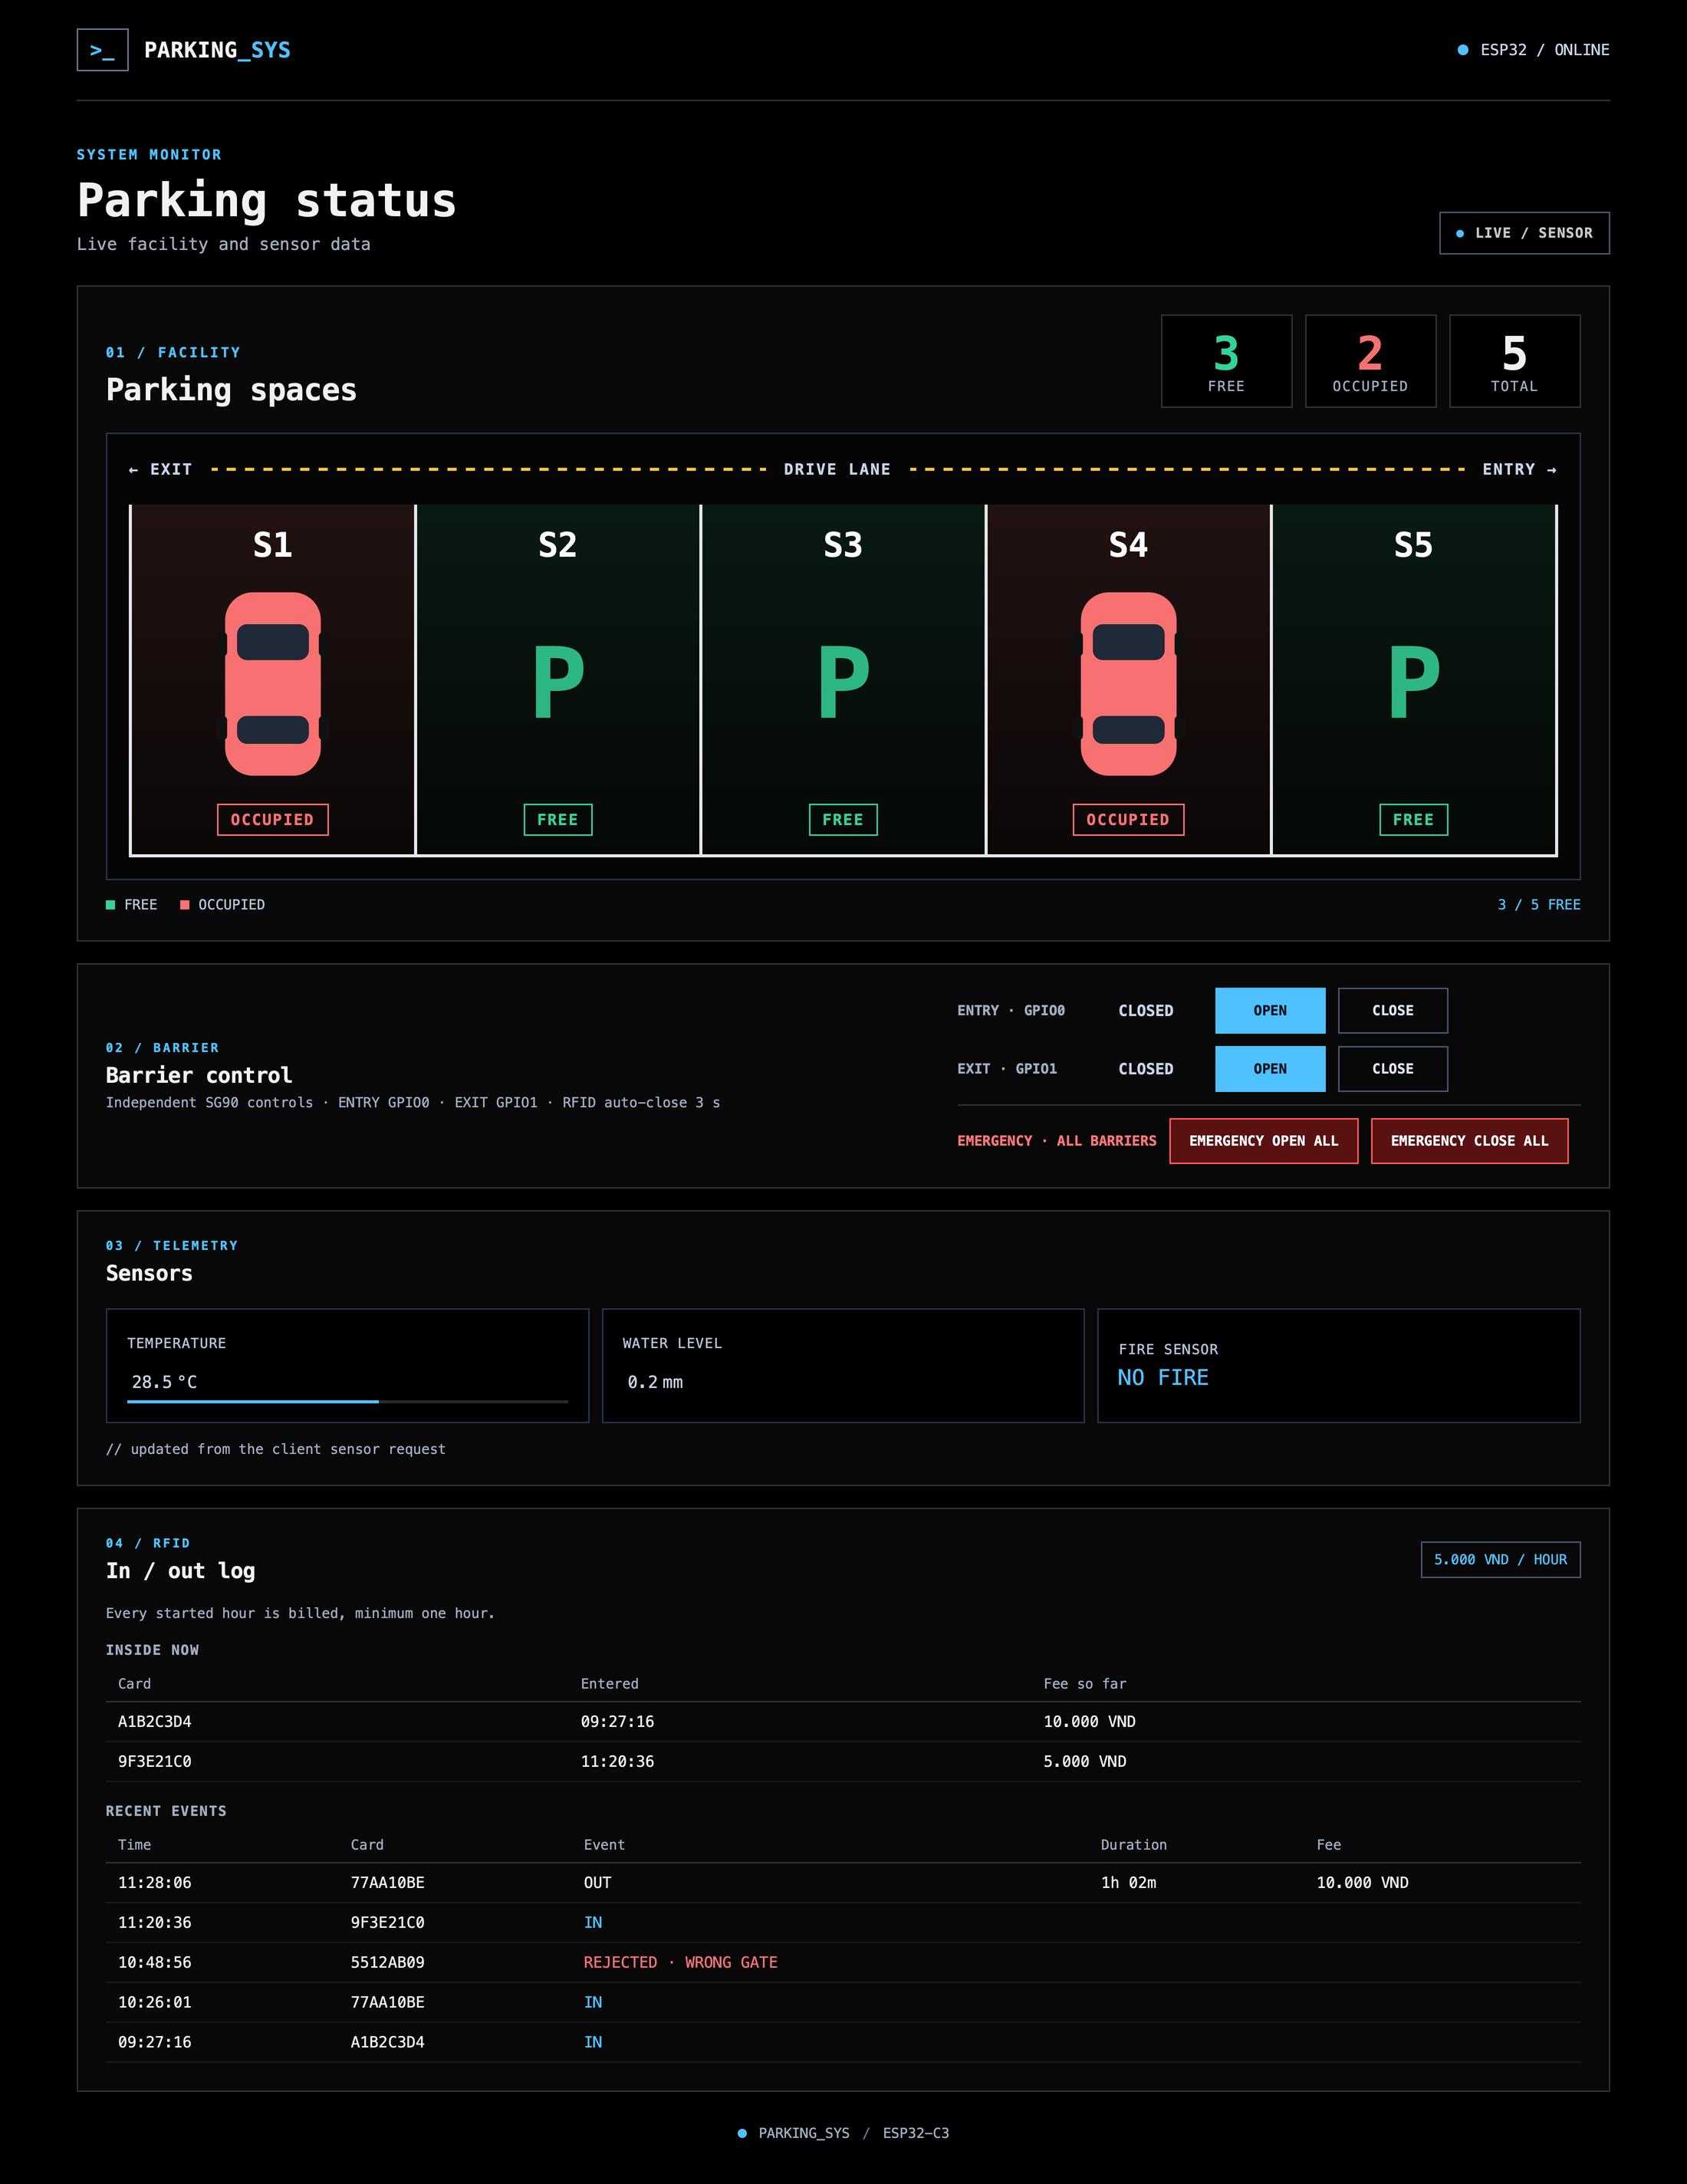
\includegraphics[width=0.86\linewidth]{dashboard.png}
\caption{Trang web giám sát tại \code{http://parking.local} (dữ liệu mẫu)}\label{fig:dashboard}
\end{figure}

\subsection{Các màn hình TFT}
\newcommand{\tftframe}[1]{%
\begin{tikzpicture}[x=0.0146cm,y=-0.0146cm,font=\tiny]
\fill[black] (0,0) rectangle (240,240);
#1
\draw[gray] (0,0) rectangle (240,240);
\end{tikzpicture}}
\newcommand{\tfttop}{%
\fill[cyan!70!blue] (0,0) rectangle (240,4);
\node[white,anchor=west,font=\tiny\bfseries] at (10,18) {PARKSENSE};
\node[gray!60,anchor=west,font=\fontsize{4}{4}\selectfont] at (10,44) {FREE SPACES};
\node[white,anchor=west,font=\scriptsize\bfseries] at (10,64) {3/5};
\fill[gray!25!black] (8,87) rectangle (68,127);
\fill[gray!25!black] (75,87) rectangle (135,127);
\node[white,anchor=west,font=\fontsize{4}{4}\selectfont] at (12,110) {28.0};
\node[white,anchor=west,font=\fontsize{4}{4}\selectfont] at (79,110) {0.2};
\fill[pink!50] (144,40) rectangle (240,136);
\foreach \i/\c in {0/red,1/green,2/green,3/red,4/green}{
  \fill[gray!25!black] (8+\i*46,147) rectangle (51+\i*46,190);
  \fill[\c] (8+\i*46,147) rectangle (11+\i*46,190);}
\fill[gray!25!black] (0,194) rectangle (240,240);}
\begin{figure}[H]
\centering
\setlength{\tabcolsep}{3pt}\begin{tabular}{cccc}
\tftframe{\tfttop
  \fill[orange!80] (90,205) rectangle (130,235);}
&
\tftframe{\tfttop
  \node[white,anchor=west,font=\fontsize{4}{4}\selectfont] at (8,201) {ID A1B2C3D4};
  \node[white,anchor=west,font=\fontsize{5}{5}\selectfont] at (8,226) {1H 01M};
  \node[cyan,anchor=west,font=\scriptsize\bfseries] at (126,222) {10000};}
&
\tftframe{\tfttop
  \node[white,anchor=west,font=\fontsize{4}{4}\selectfont] at (8,200) {ID 5512AB09};
  \node[red,anchor=west,font=\fontsize{6}{6}\selectfont\bfseries] at (8,215) {WRONG GATE};
  \node[gray!60,anchor=west,font=\fontsize{3.5}{3.5}\selectfont] at (8,232) {ALREADY INSIDE - USE EXIT GATE};}
&
\tftframe{\fill[red] (0,0) rectangle (240,8); \fill[red] (0,232) rectangle (240,240);
  \fill[red!40!black] (16,16) rectangle (224,224);
  \node[white,font=\scriptsize\bfseries] at (120,40) {DANGER};
  \fill[red] (100,90) rectangle (140,150); \fill[orange] (108,105) rectangle (132,150); \fill[yellow] (114,125) rectangle (126,150);
  \node[yellow,font=\fontsize{5}{5}\selectfont\bfseries] at (120,182) {FIRE DETECTED};
  \node[white,font=\fontsize{5}{5}\selectfont\bfseries] at (120,208) {EVACUATE NOW};}
\\[2pt]
\small (a) Bình thường & \small (b) Hóa đơn khi ra & \small (c) Quẹt sai cổng & \small (d) Có cháy \\
\end{tabular}
\caption{Bốn trạng thái màn hình TFT $240\times240$ (mô phỏng bố cục theo mã nguồn \file{lcd\_display.c})}\label{fig:tft}
\end{figure}
Trên màn hình bình thường: hàng trên là số chỗ trống, hai ô nhiệt độ và mực nước,
ảnh động $96\times96$ ở góc phải, hàng giữa là 5 ô S1–S5 với vạch xanh (trống)/đỏ (có
xe), vùng chân dùng cho ảnh động nhỏ, hóa đơn hoặc thông báo.

\subsection{Kịch bản demo}
\begin{enumerate}
\item Bật RFID Client, máy chủ, Sensor Client; mở \code{http://parking.local} trên điện thoại.
\item Đặt xe mô hình vào ô S2: ô S2 trên TFT chuyển đỏ ngay, trên web hiện hình xe trong $\le$ 1\,s.
\item Quẹt thẻ ở cổng vào: thanh chắn vào mở rồi tự đóng sau 3\,s; web có dòng \code{IN}.
\item Quẹt lại thẻ đó ở cổng vào: màn hình báo \code{WRONG GATE – ALREADY INSIDE - USE EXIT GATE}.
\item Quẹt thẻ ở cổng ra: hóa đơn hiện trên TFT, thanh chắn ra mở; web có dòng \code{OUT} kèm phí.
\item Đưa bật lửa gần cảm biến lửa: còi kêu, màn hình DANGER, hai thanh chắn mở và không đóng được từ web.
\item Tắt lửa: còi tắt, thanh chắn đóng, màn hình trở lại bình thường.
\end{enumerate}


% =====================================================================
\chapter{Hướng dẫn chạy mã nguồn từng bước}\label{chap:huongdanchay}
% =====================================================================

Chương này hướng dẫn từ lúc lấy mã nguồn đến lúc hệ thống chạy hoàn chỉnh, kèm kết
quả mong đợi ở mỗi bước để kiểm tra. Môi trường cần cài trước theo
Chương~\ref{chap:caidat}. Có hai cách chạy:
\begin{itemize}
  \item \textbf{Đầy đủ phần cứng}: Bước~1 đến Bước~9.
  \item \textbf{Không cần client} (chỉ có bo máy chủ, dùng máy tính giả lập hai client):
        Bước~1, 2, 4 rồi Bước~10.
\end{itemize}
Bộ kiểm thử tự động (không cần phần cứng nào) ở Bước~11.

\begin{table}[H]
\centering\small
\caption{Tên cổng nối tiếp theo hệ điều hành}\label{tab:ports}
\begin{tabularx}{\linewidth}{@{}lXX@{}}
\toprule
\textbf{Hệ điều hành} & \textbf{ESP32-C3 SuperMini (USB tích hợp)} & \textbf{ESP8266 NodeMCU (CH340/CP2102)} \\ \midrule
Windows & \code{COM3}, \code{COM4}, \ldots{} (xem Device Manager) & \code{COM5}, \ldots \\
macOS & \code{/dev/cu.usbmodem*} & \code{/dev/cu.usbserial-*} hoặc \code{/dev/cu.wchusbserial*} \\
Linux & \code{/dev/ttyACM0} & \code{/dev/ttyUSB0} \\
\bottomrule
\end{tabularx}
\end{table}

% ---------------------------------------------------------------------
\buoc{Lấy mã nguồn}
\begin{lstlisting}[style=shell]
git clone https://github.com/thinhdinh25/INT3108_embedded-Smart-Parking-Project.git
cd INT3108_embedded-Smart-Parking-Project
\end{lstlisting}
Hoặc tải tệp ZIP từ trang GitHub của dự án và giải nén.

\buoc{Làm quen cấu trúc thư mục}
\begin{lstlisting}[language={},numbers=none,caption={Cấu trúc kho mã nguồn}]
Server/              Firmware may chu ESP32-C3 (ESP-IDF)
  main/              Ma nguon: barrier, buzzer, display, network, parking
  sdkconfig.defaults Cau hinh mac dinh: -O2, phan vung ung dung 1,5 MB
SensorClient/        Sketch Arduino cho Sensor Client (ESP8266)
RFIDClient/          Sketch Arduino cho RFID Client (ESP8266)
examples/            Cong cu gia lap client bang Python
tests/               Bo kiem thu tu dong tren may tinh
docs/                Ghi chu dau day
report/              Bao cao nay (LaTeX + PDF)
\end{lstlisting}

\buoc{Lắp mạch}
Đấu dây theo Bảng~\ref{tab:pin-srv} (máy chủ) và Bảng~\ref{tab:pin-clients} (hai client).
Kiểm tra trước khi cấp nguồn:
\begin{itemize}
  \item Servo dùng nguồn 5\,V riêng, \textbf{GND nối chung} với ESP32-C3; không cấp
        servo từ chân 3V3.
  \item Màn hình ST7789 dùng 3V3; RC522 dùng 3V3 (không dùng 5\,V).
  \item Module còi không được kéo GPIO9 xuống mức thấp khi cấp nguồn (nếu không, bo
        sẽ vào chế độ nạp firmware).
\end{itemize}

\buoc{Biên dịch và nạp máy chủ ESP32-C3}
Mở terminal ESP-IDF (Chương~\ref{chap:caidat}), cắm ESP32-C3 qua USB:
\begin{lstlisting}[style=shell]
cd Server
idf.py set-target esp32c3        # chi lan dau; tao sdkconfig tu sdkconfig.defaults
idf.py build                     # lan dau tai them thanh phan espressif/mdns
idf.py -p <CONG> flash monitor   # vi du: -p COM4 hoac -p /dev/cu.usbmodem101
\end{lstlisting}
\textbf{Kết quả mong đợi} sau \code{idf.py build}:
\begin{lstlisting}[language={},numbers=none]
INT3108_Smart_Parking_Project.bin binary size 0x108890 bytes. Smallest app
partition is 0x177000 bytes. 0x6e770 bytes (29%) free.
Project build complete.
\end{lstlisting}
\textbf{Kết quả mong đợi} trên cửa sổ monitor (thoát bằng \code{Ctrl+]}):
\begin{lstlisting}[language={},numbers=none]
I (...) LCD_DISPLAY: ST7789 display started at 240x240 with 10-frame Kaoruko animation
I (...) WIFI_STA: Wi-Fi station started, connecting to SSID=ESP32-Parking...
I (...) HTTP_SERVER: HTTP server listening on port 80
I (...) UDP_SERVER: UDP server listening on port 3333
I (...) SERVER: Web interface: http://parking.local
\end{lstlisting}
Màn hình TFT hiện giao diện \code{PARKSENSE} với các giá trị \code{--.-}; hai thanh
chắn về vị trí đóng. Máy chủ sẽ báo \code{Got IP} khi RFID Client (điểm truy cập) đã
bật ở Bước~5.

\begin{lydo}[Lưu ý khi đã có cấu hình cũ]
\file{sdkconfig.defaults} chỉ được áp dụng khi chưa có tệp \file{Server/sdkconfig}.
Nếu máy đã từng build bản cũ, hãy chạy lại \code{idf.py set-target esp32c3} (tạo lại
cấu hình) hoặc chọn trong \code{idf.py menuconfig}: \emph{Compiler options → Optimize for
performance} và \emph{Partition Table → Single factory app (large), no OTA}. Lần nạp
đầu sau khi đổi bảng phân vùng phải dùng \code{idf.py flash} (nạp cả bảng phân vùng).
\end{lydo}

\buoc{Nạp RFID Client (điểm truy cập Wi-Fi)}
\begin{enumerate}
  \item Mở Arduino IDE, \emph{File → Open} tệp \file{RFIDClient/RFIDClient.ino}.
  \item \emph{Tools → Board}: \textbf{NodeMCU 1.0 (ESP-12E Module)}; \emph{Port}: cổng
        của bo (Bảng~\ref{tab:ports}); \emph{Upload Speed}: 115200.
  \item Bấm \textbf{Upload} (mũi tên). Chờ \code{Done uploading}.
  \item Mở \emph{Serial Monitor}, tốc độ \textbf{115200}.
\end{enumerate}
\textbf{Kết quả mong đợi}: dòng \code{Đã phát WiFi Hotspot!}, \code{SSID: ESP32-Parking},
\code{Địa chỉ IP của Hotspot: 192.168.4.1}, phiên bản firmware của hai đầu đọc và
\code{Hệ thống đã sẵn sàng!}. Trên monitor của máy chủ xuất hiện:
\begin{lstlisting}[language={},numbers=none]
I (...) WIFI_STA: Got IP: 192.168.4.2
I (...) SERVER: mDNS: parking.local -> 192.168.4.2
\end{lstlisting}

\buoc{Nạp Sensor Client}
Làm như Bước~5 với tệp \file{SensorClient/SensorClient.ino}. \textbf{Kết quả mong đợi}
trên Serial Monitor: \code{Connected, client IP: 192.168.4.x}, sau đó mỗi giây một dòng
\code{Sent: \{"type":"parking\_update",...\}}. Màn hình TFT hiện số chỗ trống thật.

\begin{lydo}[Nạp lại qua Wi-Fi (OTA)]
Từ lần thứ hai, khi máy tính kết nối Wi-Fi \code{ESP32-Parking}, hai client xuất hiện
trong \emph{Tools → Port} dưới dạng cổng mạng (ví dụ \code{ESP8266-RC522-DHT11}); chọn
cổng đó để nạp firmware mà không cần tháo bo khỏi mô hình.
\end{lydo}

\buoc{Bật hệ thống theo thứ tự}
Thứ tự khuyến nghị: \textbf{RFID Client} (phát Wi-Fi) → \textbf{máy chủ} → \textbf{Sensor
Client}. Thứ tự khác vẫn chạy được vì máy chủ và Sensor Client tự kết nối lại, chỉ
chậm hơn vài giây.

\buoc{Mở trang web giám sát}
\begin{enumerate}
  \item Trên điện thoại/máy tính, kết nối Wi-Fi \code{ESP32-Parking}, mật khẩu \code{12345678}.
  \item Mở trình duyệt, vào \code{http://parking.local}.
  \item Nếu thiết bị không mở được tên \code{.local} (một số máy Android cũ), dùng địa chỉ
        IP trong dòng \code{Web interface: http://192.168.4.x} trên monitor của máy chủ.
\end{enumerate}
\textbf{Kết quả mong đợi}: trang như Hình~\ref{fig:dashboard}, góc trên phải hiện
\code{ESP32 / ONLINE} và nhãn \code{LIVE / SENSOR}.

\buoc{Chạy các kịch bản demo}
Thực hiện kịch bản ở mục~\ref{sec:demo} và đối chiếu với Bảng~\ref{tab:systest}
(Chương~\ref{chap:kiemthu}).

\buoc{Chạy khi không có hai client (giả lập bằng máy tính)}
\begin{enumerate}
  \item Tạo điểm phát Wi-Fi trên điện thoại với tên \code{ESP32-Parking}, mật khẩu
        \code{12345678} (máy chủ sẽ tự kết nối vào), \emph{hoặc} dùng RFID Client nếu có.
  \item Cho máy tính kết nối cùng Wi-Fi; mở monitor máy chủ để xem IP
        (\code{Got IP: \ldots}).
  \item Giả lập Sensor Client và RFID Client (thay \code{<IP>} bằng IP máy chủ; nếu dùng
        RFID Client làm điểm phát thì có thể bỏ \code{--host}):
\end{enumerate}
\begin{lstlisting}[style=shell]
python3 examples/udp_sender.py --host <IP> --slots 1,0,0,1,0
python3 examples/udp_rfid_sender.py A1B2C3D4 --gate in  --host <IP>
python3 examples/udp_rfid_sender.py A1B2C3D4 --gate in  --host <IP>  # quet lai: WRONG GATE
python3 examples/udp_rfid_sender.py A1B2C3D4 --gate out --host <IP>  # ra: hoa don
python3 examples/udp_sender.py --host <IP> --slots 1,0,0,1,0 --fire  # bao chay
python3 examples/udp_sender.py --host <IP> --slots 1,0,0,1,0         # het chay
\end{lstlisting}
\textbf{Kết quả mong đợi}: TFT và trang web thay đổi đúng như khi dùng client thật;
thanh chắn mở/đóng; nhật ký trên web có các dòng \code{IN}, \code{REJECTED · WRONG GATE},
\code{OUT}. Trên Windows dùng \code{python} thay cho \code{python3}.

\buoc{Chạy bộ kiểm thử tự động}
Không cần ESP-IDF hay Arduino, chỉ cần trình biên dịch C/C++:
\begin{lstlisting}[style=shell]
make -C tests
\end{lstlisting}
\textbf{Kết quả mong đợi}:
\begin{lstlisting}[language={},numbers=none]
json_parsers             57/57 checks passed
rfid_session             74/74 checks passed
gif_frames               89/89 checks passed
sensor_client            15/15 checks passed
rfid_client              15/15 checks passed
ALL TESTS PASSED
\end{lstlisting}

\section{Xử lý sự cố thường gặp}
\begin{longtable}{@{}p{4.6cm}p{9.8cm}@{}}
\caption{Lỗi thường gặp và cách khắc phục}\label{tab:troubleshoot}\\
\toprule \textbf{Hiện tượng} & \textbf{Nguyên nhân và cách khắc phục} \\ \midrule \endfirsthead
\toprule \textbf{Hiện tượng} & \textbf{Nguyên nhân và cách khắc phục} \\ \midrule \endhead
\code{idf.py: command not found} & Chưa mở terminal ESP-IDF; mở shortcut/script kích hoạt do EIM tạo. \\
\code{Failed to connect to ESP32-C3} & Sai cổng; hoặc giữ nút BOOT, bấm RESET, thả BOOT rồi nạp lại. \\
Build báo phân vùng đầy & Đang dùng \file{sdkconfig} cũ (1\,MB): làm theo hộp ``Lưu ý khi đã có cấu hình cũ'' ở Bước~4. \\
Monitor lặp \code{Disconnected ... retrying} & RFID Client chưa bật hoặc sai SSID/mật khẩu; kiểm tra Bước~5. \\
Arduino không thấy cổng ESP8266 & Cài driver CH340/CP2102; thử cáp USB khác (cáp chỉ sạc không truyền dữ liệu). \\
Thiếu \code{MFRC522.h} hoặc \code{DHT.h} & Cài thư viện như Chương~\ref{chap:caidat}. \\
\code{parking.local} không mở & Thiết bị không hỗ trợ mDNS: dùng IP trong log máy chủ; kiểm tra điện thoại đang ở đúng Wi-Fi \code{ESP32-Parking}. \\
Trang web báo \code{OFFLINE} & Máy chủ mất điện hoặc mất Wi-Fi; xem monitor máy chủ. \\
Servo rung, bo tự khởi động lại & Cấp servo từ 3V3 hoặc thiếu GND chung; dùng nguồn 5\,V riêng. \\
Màn hình trắng hoặc lệch hình & Kiểm tra dây SPI; chỉnh chân/độ lệch trong \code{idf.py menuconfig → Parking TFT display}. \\
Ô đỗ báo ngược (trống thành có xe) & Chỉnh biến trở trên module IR; kiểm tra thứ tự chân S1–S5. \\
\bottomrule
\end{longtable}

% =====================================================================
\chapter{Kiểm thử}\label{chap:kiemthu}
% =====================================================================

\section{Chiến lược kiểm thử}
\begin{figure}[H]
\centering
\mmd[0.92][0.6]{testpyramid}
\caption{Ba tầng kiểm thử: càng xuống dưới càng nhanh, tự động và chạy thường xuyên}\label{fig:testpyramid}
\end{figure}

\section{Kiểm thử tự động}
Bộ kiểm thử nằm trong \file{tests/} và chạy bằng \code{make -C tests}. Các module
nghiệp vụ của máy chủ được biên dịch với hai header giả (critical section và đồng hồ
điều khiển được). Hai sketch Arduino được biên dịch \emph{nguyên vẹn} cùng lớp giả lập
thư viện (\file{tests/arduino/}): đồng hồ \code{millis()}, mức logic từng chân, ADC,
Wi-Fi, UDP, đầu đọc MFRC522 và DHT11.

\begin{table}[H]
\centering\small
\caption{Các bộ kiểm thử tự động và kết quả}\label{tab:unittests}
\begin{tabularx}{\linewidth}{@{}lXr@{}}
\toprule
\textbf{Bộ} & \textbf{Nội dung kiểm tra} & \textbf{Kết quả} \\ \midrule
\file{json\_parsers} & Bản tin hợp lệ (mọi thứ tự khóa, khoảng trắng, giới hạn dải); 22 bản tin \code{parking\_update} sai và 16 bản tin \code{rfid\_event} sai đều bị từ chối (thiếu/thừa khóa, khóa lặp, sai kiểu, ngoài dải, ký tự lạ, dữ liệu thừa, chuỗi có ký tự thoát) & 57/57 \\
\file{rfid\_session} & Phí theo giờ (biên 0, 3600, 3601\,s, bão hòa); vào/ra, sai cổng; hóa đơn hết hạn đúng 60\,s; bãi đầy, tái sử dụng chỗ; nhiệt độ; nhật ký vòng (thứ tự, chỉ giữ 10); thông báo từ chối 5\,s & 74/74 \\
\file{gif\_frames} & 28 khung ảnh động giải nén đủ; nền đã xóa và byte đã đảo đúng; từ chối yêu cầu sai kích thước & 89/89 \\
\file{sensor\_client} & Chạy \file{SensorClient.ino}: nhắc lại đúng 1 gói/giây; gửi ngay sau 50\,ms khi có xe; lọc nhiễu 30\,ms; thứ tự S1–S5; báo cháy và hết cháy; quy đổi mực nước; mất/có lại Wi-Fi; mọi gói được bộ đọc của máy chủ chấp nhận & 15/15 \\
\file{rfid\_client} & Chạy \file{RFIDClient.ino}: UID hex in hoa; cổng vào/ra; chống lặp 2\,s trên cả hai đầu đọc; UID 10 byte; DHT11 lỗi giữ giá trị cũ; mọi gói được bộ đọc của máy chủ chấp nhận & 15/15 \\ \midrule
\textbf{Tổng} & & \textbf{250/250} \\
\bottomrule
\end{tabularx}
\end{table}

\begin{lstlisting}[language=C,caption={[Ví dụ kiểm thử chống rung của Sensor Client]Ví dụ kiểm thử chống rung của Sensor Client (\file{tests/test\_sensor\_client.cpp})}]
/* A car on S1 is reported as soon as the 50 ms debounce passes. */
fake::pin_level[SLOT_PINS[0]] = LOW;
run_for(40);
CHECK(fake::udp_sent.empty());            /* still inside the debounce window */
run_for(30);
CHECK(fake::udp_sent.size() == 1);
CHECK(last_packet(&s) && s.slots[0] == 1); /* parsed by the real server parser */
\end{lstlisting}

\begin{lydo}[Tại sao kiểm thử trên máy tính]
Lỗi trong bộ đọc bản tin, cách tính phí hay logic chống rung rất khó tái hiện trên
phần cứng (phải đúng thời điểm, đúng chuỗi byte). Trên máy tính, đồng hồ giả cho phép
kiểm tra chính xác đến từng mili giây, cả bộ chạy trong vài giây và chạy lại sau mỗi
lần sửa mã. Việc đưa gói tin của client vào bộ đọc thật của máy chủ bảo đảm hai bên
luôn khớp định dạng — lỗi kiểu ``client gửi \code{temperature\_c} trong
\code{parking\_update} bị máy chủ từ chối'' được phát hiện ngay.
\end{lydo}

Bộ kiểm thử cũng đã giúp phát hiện một lỗi \emph{trong chính bài kiểm thử}: khi kiểm
tra ``bãi đầy'', một thẻ từ bài kiểm thử trước vẫn còn trong bãi khiến chỉ còn 4 chỗ
trống. Bài kiểm thử được sửa để tự dọn trạng thái — đúng như mục đích của việc chạy
kiểm thử thường xuyên.

\section{Kiểm thử tích hợp bằng công cụ giả lập}
Các lệnh ở Bước~10 (Chương~\ref{chap:huongdanchay}) gửi bản tin thật tới máy chủ thật;
dùng để kiểm tra màn hình, thanh chắn, còi, trang web và nhật ký khi chưa có đủ client.

\section{Kịch bản kiểm thử hệ thống trên phần cứng}
\begin{longtable}{@{}p{0.9cm}>{\raggedright\arraybackslash}p{5.6cm}>{\raggedright\arraybackslash}p{7.9cm}@{}}
\caption{Kịch bản kiểm thử trên phần cứng và hành vi mong đợi}\label{tab:systest}\\
\toprule \textbf{\#} & \textbf{Thao tác} & \textbf{Hành vi mong đợi} \\ \midrule \endfirsthead
\toprule \textbf{\#} & \textbf{Thao tác} & \textbf{Hành vi mong đợi} \\ \midrule \endhead
S1 & Cấp nguồn RFID Client, rồi máy chủ & Có Wi-Fi \code{ESP32-Parking}; máy chủ báo \code{Got IP} và \code{mDNS: parking.local -> ...}; TFT hiện giao diện; hai thanh chắn đóng \\
S2 & Cấp nguồn Sensor Client, mở \code{parking.local} & Web hiện sơ đồ 5 ô, \code{LIVE / SENSOR} \\
S3 & Đặt xe vào ô S2 & TFT đổi ô S2 sang đỏ gần như tức thì; web hiện hình xe ở S2 trong $\le$ 1\,s \\
S4 & Rê vật nhanh qua cảm biến ($<$ 50\,ms) & Trạng thái không đổi \\
S5 & Quẹt thẻ mới ở cổng vào & Thanh chắn vào mở, tự đóng sau 3\,s; web có dòng \code{IN}; nhiệt độ cập nhật \\
S6 & Giữ thẻ trên đầu đọc 1\,s & Chỉ một sự kiện được gửi \\
S7 & Quẹt lại thẻ đó ở cổng vào & Không mở; TFT \code{WRONG GATE – ALREADY INSIDE - USE EXIT GATE} 5\,s; web \code{REJECTED · WRONG GATE} \\
S8 & Quẹt thẻ đó ở cổng ra & Thanh chắn ra mở; TFT hiện hóa đơn 60\,s; web \code{OUT} kèm thời lượng và phí \\
S9 & Đưa lửa gần cảm biến lửa & Còi kêu; TFT \code{DANGER}; hai thanh chắn mở; băng rôn đỏ trên web \\
S10 & Bấm \code{CLOSE} trên web khi đang cháy & Bị từ chối, thanh chắn vẫn mở \\
S11 & Tắt lửa & Còi tắt, hai thanh chắn đóng, TFT trở lại bình thường \\
S12 & Bấm \code{OPEN}/\code{CLOSE}/\code{EMERGENCY} trên web & Thanh chắn tương ứng chuyển động, trạng thái trên web đúng \\
S13 & Quẹt thẻ thứ 6 khi đã có 5 xe & Không mở; TFT \code{PARKING FULL} \\
S14 & Tắt RFID Client rồi bật lại & Máy chủ và Sensor Client tự kết nối lại; \code{parking.local} trỏ đúng IP mới \\
S15 & Gửi gói UDP rác từ máy tính & Máy chủ ghi cảnh báo và tiếp tục hoạt động \\
\bottomrule
\end{longtable}

% =====================================================================
\chapter{Tổng kết}\label{chap:ketluan}
% =====================================================================

\section{Kết quả đạt được}
Nhóm đã xây dựng hoàn chỉnh một hệ thống bãi đỗ xe thông minh quy mô mô hình gồm ba
vi điều khiển, tự vận hành trên mạng Wi-Fi riêng:
\begin{itemize}
  \item \textbf{10 use case} (Chương~\ref{chap:usecase}) đều được hiện thực: theo dõi chỗ
        trống tại bãi và trên web, gửi/lấy xe bằng RFID kèm tính phí, từ chối quẹt sai
        cổng hoặc bãi đầy, cảnh báo cháy và mở đường sơ tán, giám sát nước và nhiệt độ,
        điều khiển thanh chắn thủ công, nhật ký vào/ra kèm giá.
  \item \textbf{Kiến trúc} phân lớp rõ ràng, không vòng phụ thuộc; đa tác vụ với
        FreeRTOS và ba cơ chế đồng bộ dùng đúng chỗ; giao tiếp UDP nhẹ, tự sửa khi mất gói;
        tên \code{parking.local} luôn trỏ đúng IP.
  \item \textbf{Hiệu năng}: màn hình phản ánh thay đổi trong khoảng 0,1\,s; thanh chắn mở
        khoảng 0,2\,s sau khi quẹt thẻ; firmware dùng 36\% RAM tĩnh, còn 29\% flash ứng dụng.
  \item \textbf{Chất lượng}: 250 phép kiểm thử tự động đều đạt, chạy cả mã nguồn hai
        client trên phần cứng giả lập.
\end{itemize}

Qua đề tài, nhóm đã vận dụng các kiến thức trọng tâm của môn lập trình nhúng: hệ điều
hành thời gian thực, đồng bộ tác vụ, PWM và SPI có DMA, ADC và lọc nhiễu tín hiệu số,
lập trình socket, quản lý bộ nhớ hạn chế, xử lý dữ liệu không tin cậy, và kiểm thử
phần mềm nhúng không cần phần cứng.

\section{Hạn chế}
\begin{enumerate}
  \item \textbf{Bảo mật}: bản tin UDP và API điều khiển chưa có xác thực; mật khẩu Wi-Fi
        cố định trong mã nguồn.
  \item \textbf{Sự kiện RFID có thể mất}: khác bản tin cảm biến, sự kiện quẹt thẻ không
        được nhắc lại; nếu gói bị mất, người lái phải quẹt lại.
  \item \textbf{Dữ liệu trong RAM}: phiên gửi xe và nhật ký mất khi máy chủ khởi động lại;
        thời gian tính từ lúc khởi động, không phải giờ thực.
  \item \textbf{Nhiệt độ} chỉ được cập nhật khi có xe quẹt thẻ (đi kèm bản tin RFID).
  \item \textbf{Số phiên RFID và cảm biến IR} chưa được đối chiếu với nhau.
\end{enumerate}

\section{Hướng phát triển}
\begin{itemize}
  \item Thêm mã xác thực HMAC-SHA256 (có sẵn trong mbedTLS của ESP-IDF) và số thứ tự chống
        phát lại cho mỗi bản tin; thêm đăng nhập cho API điều khiển.
  \item Bản tin xác nhận (ACK) cho \code{rfid\_event}; RFID Client gửi lại nếu không nhận được.
  \item Lưu phiên vào NVS theo lô; đồng bộ giờ bằng SNTP hoặc module RTC DS3231.
  \item Gửi nhiệt độ định kỳ độc lập với sự kiện quẹt thẻ.
  \item Kết nối MQTT lên đám mây để quản lý nhiều bãi, thống kê doanh thu, đặt chỗ trước,
        thanh toán bằng mã QR.
  \item Bổ sung OTA cho máy chủ (bảng phân vùng hai khe ứng dụng).
\end{itemize}

% =====================================================================
\chapter{Đóng góp của thành viên và phân chia điểm}\label{chap:donggop}
% =====================================================================

\section{Cách nhóm chia việc}
Đề tài có ba mảng khối lượng tương đương: \textbf{phần mềm} (firmware ba bo mạch,
trang web, kiểm thử), \textbf{điện} (chọn linh kiện, nguồn, đi dây) và \textbf{cơ khí}
(mô hình, cơ cấu thanh chắn). Mỗi thành viên phụ trách chính một mảng và tham gia
phần giao giữa các mảng: người làm điện viết firmware đọc cảm biến mình lắp, người làm
mô hình viết firmware điều khiển servo mình gắn. Nhóm làm việc trên một kho GitHub
chung từ 22/09 đến 30/10/2026, họp mỗi tuần để tích hợp và chạy thử trên mô hình.

\begin{table}[H]
\centering\small
\caption{Mảng phụ trách chính}\label{tab:mang}
\begin{tabularx}{\linewidth}{@{}lXX@{}}
\toprule
\textbf{Thành viên} & \textbf{Mảng chính} & \textbf{Phần giao với mảng khác} \\ \midrule
Nguyễn Chí Minh & Phần mềm: firmware máy chủ, trang web, giao thức, bảo mật, kiểm thử & Tích hợp firmware hai client vào giao thức chung; tối ưu toàn hệ thống \\
Đinh Đức Thịnh & Điện: chọn phần cứng, thiết kế nguồn, sơ đồ chân, đi dây & Firmware RFID Client và Sensor Client; khởi tạo dự án ESP-IDF \\
Nguyễn Việt Tiến & Cơ khí: mô hình bãi xe, cơ cấu thanh chắn servo & Firmware thanh chắn và còi; tài liệu hướng dẫn cài đặt \\
\bottomrule
\end{tabularx}
\end{table}

\section{Chi tiết đóng góp từng thành viên}

\subsection{Nguyễn Chí Minh (24020232) — phần mềm và tích hợp}
\begin{itemize}
  \item \textbf{Firmware máy chủ ESP32-C3}: dựng kiến trúc phân lớp, các tác vụ FreeRTOS
        và cơ chế đồng bộ; UDP server, HTTP server với 12 route; mDNS
        \code{parking.local} tự thông báo lại khi đổi IP; xử lý lỗi \code{accept (23)}
        bằng giới hạn và thu hồi kết nối.
  \item \textbf{Màn hình ST7789}: driver SPI có DMA, giao diện \code{PARKSENSE}, hóa đơn,
        thông báo quẹt sai cổng, màn hình cháy; nén ảnh động LZSS và tiền xử lý trên máy
        tính để giảm RAM và CPU.
  \item \textbf{Giao thức và bảo mật}: định dạng JSON và bộ đọc JSON không cấp phát động;
        ký gói SipHash-2-4, cửa sổ chống phát lại, ACK cho sự kiện quẹt thẻ; mã PIN cho
        API; lưu phiên vào NVS và đồng hồ bãi lấy giờ từ trình duyệt.
  \item \textbf{Trang web giám sát}: sơ đồ bãi trực quan, điều khiển thanh chắn, nhật ký
        vào/ra kèm phí, cảnh báo lệch thẻ/cảm biến.
  \item \textbf{Kiểm thử}: lớp giả lập Arduino để chạy nguyên mã hai sketch trên máy tính;
        6 bộ kiểm thử, 318 phép kiểm tra; công cụ giả lập client bằng Python.
  \item \textbf{Báo cáo}: Chương 3, 5 và các sơ đồ Mermaid.
\end{itemize}
\textit{Các commit tiêu biểu}:
\begin{itemize}[nosep]
  \item \code{init server}, \code{add udp server}, \code{add display st7789},
        \code{add kaoruko anime gif to display}, \code{add emergency button};
  \item \code{update dashboard UI and display UI, fix rgb565 byte swap logic};
  \item \code{Add parking.local mDNS}, \code{Optimize firmware, add host tests},
        \code{Fix HTTP accept failures}.
\end{itemize}

\subsection{Đinh Đức Thịnh (24020313) — điện, phần cứng và client}
\begin{itemize}
  \item \textbf{Lựa chọn phần cứng}: so sánh và chốt ESP32-C3 SuperMini cho máy chủ,
        ESP8266 cho client; cảm biến IR HW-201, module lửa, cảm biến mực nước, RC522,
        DHT11 theo tiêu chí giá, mức logic 3,3\,V và số chân (Bảng~\ref{tab:sensors}).
  \item \textbf{Thiết kế nguồn}: một điểm cấp nguồn qua jack DC trên vách sau; diode
        chống cắm ngược cực; tụ hóa lọc sụt áp khi servo khởi động — nguyên nhân làm
        ESP32-C3 tự reset ở bản lắp thử đầu tiên; tách nguồn 5\,V cho servo, nối chung GND.
  \item \textbf{Sơ đồ chân và đi dây}: lập sơ đồ chân ba bo tránh chân strapping và UART
        (Bảng~\ref{tab:pin-srv}, \ref{tab:pin-clients}); gắn 5 module IR và module lửa ở
        mặt ngoài vách để dây không đi qua lòng bãi; đổi chân GPIO client khi phát hiện
        xung đột lúc khởi động (commit \code{Change some client GPIO}); chỉnh biến trở
        từng module IR theo độ phản xạ của xe mẫu.
  \item \textbf{Firmware client}: Sensor Client đọc 5 IR, lửa, mực nước; RFID Client với
        hai đầu đọc RC522 dùng chung SPI bật/tắt ăng-ten luân phiên để tránh nhiễu chéo,
        DHT11, điểm truy cập Wi-Fi, OTA; logic vào/ra theo cổng ở máy chủ.
  \item \textbf{Báo cáo}: Chương 2, 4 và phần nguồn điện, sơ đồ chân.
\end{itemize}
\textit{Các commit tiêu biểu}: \code{Init New ESP-IDF Project},
\code{Restructure ESP32 server and add client sketch}, \code{Change some client GPIO},
\code{Update client RFID}, \code{Complete RFID in and out logic}.

\subsection{Nguyễn Việt Tiến (24020322) — mô hình và thanh chắn}
\begin{itemize}
  \item \textbf{Mô hình bãi xe} (Hình~\ref{fig:model}): thiết kế kích thước 5 ô đỗ và hai
        làn theo chiều dài xe mẫu; cắt, dán đế và vách bằng bìa formex; khoét lỗ cho đầu
        phát/thu của cảm biến đúng giữa từng ô; làm hộp điều khiển trung tâm có ô cho màn
        hình, hai hông gắn đầu đọc RC522, nóc gắn DHT11.
  \item \textbf{Cơ cấu thanh chắn}: gắn hai servo SG90 ở đầu vách, làm cần chắn nhẹ để
        servo không quá tải; căn góc đóng/mở thực tế cho hai cổng lắp đối xứng (commit
        \code{reverse door}: cổng ra quay ngược chiều cổng vào).
  \item \textbf{Firmware thanh chắn và còi}: điều khiển hai servo bằng LEDC, tự đóng sau
        khi mở bằng thẻ, chế độ mở khi cháy (commit \code{Add dual SG90 barrier control and
        test sketch}, \code{update automated door}); module còi báo cháy
        (\code{implement buzzer}).
  \item \textbf{Tài liệu và kiểm thử phần cứng}: README hướng dẫn cài đặt
        (\code{docs: add project setup README}); kịch bản kiểm thử trên mô hình
        (Bảng~\ref{tab:systest}) và quay video demo.
  \item \textbf{Báo cáo}: Chương 1, 6, 7, 8.
\end{itemize}

\subsection{Cả nhóm}
Phân tích yêu cầu và 10 use case; thống nhất giao thức giữa ba bo; các buổi tích hợp
trên mô hình (tinh chỉnh thời gian lọc nhiễu IR từ 250\,ms xuống 50\,ms, thời gian mở
cổng từ 5\,s xuống 3\,s, thứ tự ô S1–S5); rà soát chéo báo cáo.

\section{Lịch sử đóng góp trên GitHub}
\begin{table}[H]
\centering\small
\caption{Các mốc chính trong lịch sử commit}\label{tab:timeline}
\begin{tabularx}{\linewidth}{@{}llX@{}}
\toprule
\textbf{Thời gian} & \textbf{Thành viên} & \textbf{Nội dung} \\ \midrule
22–25/09 & Thịnh & Khởi tạo dự án ESP-IDF, thử nghiệm bo mạch \\
29/09–08/10 & Minh & Khung máy chủ, UDP, HTTP, màn hình ST7789, trang web \\
02/10 & Thịnh & Tổ chức lại thư mục máy chủ, sketch client đầu tiên \\
13–20/10 & Minh, Thịnh & Định dạng bản tin, logic cảm biến IR, đổi chân GPIO client \\
20–27/10 & Tiến & Hai thanh chắn servo, tự đóng, còi, README \\
27–30/10 & Thịnh & RFID Client hai đầu đọc, logic vào/ra theo cổng \\
29–30/10 & Minh & Tối ưu, mDNS, kiểm thử, bảo mật, lưu NVS, báo cáo \\
\bottomrule
\end{tabularx}
\end{table}

Số commit không phản ánh đầy đủ khối lượng công việc: phần điện (chọn linh kiện, đo
đạc, đi dây, sửa lỗi nguồn) và phần cơ khí (chế tạo mô hình, căn chỉnh servo) chiếm
nhiều thời gian nhưng không nằm trong Git. Vì vậy nhóm đánh giá đóng góp theo mảng
việc và thời gian bỏ ra, không theo số dòng mã.

\section{Tỉ lệ đóng góp và phân chia điểm}
Cả ba thành viên thống nhất rằng \textbf{mức đóng góp là ngang nhau}. Theo quy định
của môn học, toàn bộ thành viên nhận 100\% số điểm của báo cáo.

\begin{table}[H]
\centering\small
\caption{Tỉ lệ đóng góp và tỉ lệ điểm}\label{tab:diem}
\begin{tabular}{@{}llcc@{}}
\toprule
\textbf{Thành viên} & \textbf{MSSV} & \textbf{Tỉ lệ đóng góp} & \textbf{Tỉ lệ điểm báo cáo} \\ \midrule
Nguyễn Chí Minh & 24020232 & 33,3\% & 100\% \\
Đinh Đức Thịnh & 24020313 & 33,3\% & 100\% \\
Nguyễn Việt Tiến & 24020322 & 33,3\% & 100\% \\
\bottomrule
\end{tabular}
\end{table}

\vspace{1cm}
\noindent Xác nhận của các thành viên:
\par\vspace{0.5cm}
\noindent
\begin{tabular*}{\linewidth}{@{\extracolsep{\fill}}ccc@{}}
Nguyễn Chí Minh & Đinh Đức Thịnh & Nguyễn Việt Tiến \\[1.6cm]
\rule{3.6cm}{0.4pt} & \rule{3.6cm}{0.4pt} & \rule{3.6cm}{0.4pt} \\
\end{tabular*}


% =====================================================================
\chapter*{Tài liệu tham khảo}
\addcontentsline{toc}{chapter}{Tài liệu tham khảo}
\begin{enumerate}[label={[\arabic*]}]
\item Espressif Systems, \emph{ESP32-C3 Series Datasheet} và \emph{ESP32-C3 Technical
  Reference Manual}.
\item Espressif Systems, \emph{ESP-IDF Programming Guide} (v6.1): Wi-Fi, LEDC, SPI
  Master, LCD, NVS, HTTP Server, ESP Timer, FreeRTOS, Partition Tables.
\item Espressif Systems, \emph{mDNS component} (\code{espressif/mdns}), ESP Component
  Registry.
\item Espressif Systems, \emph{ESP8266EX Datasheet}.
\item ESP8266 Community, \emph{ESP8266 Arduino Core Documentation}.
\item Sitronix, \emph{ST7789V — 240RGB$\times$320 dot 262K Color TFT Controller}.
\item NXP Semiconductors, \emph{MFRC522 Standard Performance MIFARE and NTAG
  Frontend}, Product Data Sheet.
\item TowerPro, \emph{SG90 Micro Servo Datasheet}.
\item Aosong, \emph{DHT11 Humidity \& Temperature Sensor Datasheet}.
\item R.~Barry, \emph{Mastering the FreeRTOS Real Time Kernel}, Real Time Engineers Ltd.
\item S.~Cheshire, M.~Krochmal, \emph{RFC 6762: Multicast DNS}, IETF, 2013.
\item J.~A.~Storer, T.~G.~Szymanski, ``Data compression via textual substitution'',
  \emph{Journal of the ACM}, 29(4), 1982.
\item Thư viện \emph{MFRC522} (miguelbalboa) và \emph{DHT sensor library} (Adafruit)
  cho Arduino.
\end{enumerate}

\end{document}
